%&preformat-present

\newif\ifpresentation % Условие, проверяющее, что документ --- презентация
\presentationtrue
\documentclass[10pt, xcolor={dvipsnames, table, hyperref}]{beamer}

%%%%%%%%%%%%%%%%%%%%%%%%%%%%%%%%%%%%%%%%%%%%%%%%%%%%%%%%%%%%%%%%%%%%%%%%%%%%%%%%
%%%% Файл упрощённых настроек шаблона, общих для диссертации и автореферата %%%%
%%%%%%%%%%%%%%%%%%%%%%%%%%%%%%%%%%%%%%%%%%%%%%%%%%%%%%%%%%%%%%%%%%%%%%%%%%%%%%%%

%%% Режим черновика %%%
\makeatletter
\@ifundefined{c@draft}{
  \newcounter{draft}
  \setcounter{draft}{0}  % 0 --- чистовик (максимальное соблюдение ГОСТ)
                         % 1 --- черновик (отклонения от ГОСТ, но быстрая
                         %       сборка итоговых PDF)
}{}
\makeatother

%%% Пометки в тексте %%%
\makeatletter
\@ifundefined{c@showmarkup}{
  \newcounter{showmarkup}
  \setcounter{showmarkup}{0}  % 0 --- скрыть пометки
                              % 1 --- показывать пометки
}{}
\makeatother

%%% Использование в pdflatex шрифтов не по-умолчанию %%%
\makeatletter
\@ifundefined{c@usealtfont}{
  \newcounter{usealtfont}
  \setcounter{usealtfont}{1}    % 0 --- шрифты на базе Computer Modern
                                % 1 --- использовать пакет pscyr, при его
                                %       наличии
                                % 2 --- использовать пакет XCharter, при наличии
                                %       подходящей версии
}{}
\makeatother

%%% Использование в xelatex и lualatex семейств шрифтов %%%
\makeatletter
\@ifundefined{c@fontfamily}{
  \newcounter{fontfamily}
  \setcounter{fontfamily}{1}  % 0 --- CMU семейство. Используется как fallback;
                              % 1 --- Шрифты от MS (Times New Roman и компания)
                              % 2 --- Семейство Liberation
}{}
\makeatother

%%% Библиография %%%
\makeatletter
\@ifundefined{c@bibliosel}{
  \newcounter{bibliosel}
  \setcounter{bibliosel}{0}   % 0 --- встроенная реализация с загрузкой файла
                              %       через движок bibtex8;
                              % 1 --- реализация пакетом biblatex через движок
                              %       biber
}{}
\makeatother

%%% Вывод типов ссылок в библиографии %%%
\makeatletter
\@ifundefined{c@mediadisplay}{
  \newcounter{mediadisplay}
  \setcounter{mediadisplay}{1}   % 0 --- не делать ничего; надписи [Текст] и
                                 %       [Эл. ресурс] будут выводиться только в ссылках с
                                 %       заполненным полем `media`;
                                 % 1 --- автоматически добавлять надпись [Текст] к ссылкам с
                                 %       незаполненным полем `media`; таким образом, у всех
                                 %       источников будет указан тип, что соответствует
                                 %       требованиям ГОСТ
                                 % 2 --- автоматически удалять надписи [Текст], [Эл. Ресурс] и др.;
                                 %       не соответствует ГОСТ
                                 % 3 --- автоматически удалять надпись [Текст];
                                 %       не соответствует ГОСТ
                                 % 4 --- автоматически удалять надпись [Эл. Ресурс];
                                 %       не соответствует ГОСТ
}{}
\makeatother

%%% Предкомпиляция tikz рисунков для ускорения работы %%%
\makeatletter
\@ifundefined{c@imgprecompile}{
  \newcounter{imgprecompile}
  \setcounter{imgprecompile}{0}   % 0 --- без предкомпиляции;
                                  % 1 --- пользоваться предварительно
                                  %       скомпилированными pdf вместо генерации
                                  %       заново из tikz
}{}
\makeatother
               % Общие настройки шаблона
\input{common/packages}            % Пакеты общие для диссертации и автореферата
%%% Основные сведения %%%
\newcommand{\thesisAuthorLastName}{Булатов}
\newcommand{\thesisAuthorOtherNames}{Виктор Геннадьевич}
\newcommand{\thesisAuthorInitials}{В.\,Г.}
\newcommand{\thesisAuthor}             % Диссертация, ФИО автора
{%
    \texorpdfstring{% \texorpdfstring takes two arguments and uses the first for (La)TeX and the second for pdf
        \thesisAuthorLastName~\thesisAuthorOtherNames% так будет отображаться на титульном листе или в тексте, где будет использоваться переменная
    }{%
        \thesisAuthorLastName, \thesisAuthorOtherNames% эта запись для свойств pdf-файла. В таком виде, если pdf будет обработан программами для сбора библиографических сведений, будет правильно представлена фамилия.
    }
}
\newcommand{\thesisAuthorShort}        % Диссертация, ФИО автора инициалами
{\thesisAuthorInitials~\thesisAuthorLastName}
%\newcommand{\thesisUdk}                % Диссертация, УДК
%{\fixme{xxx.xxx}}
\newcommand{\thesisTitle}              % Диссертация, название
{Методы оценивания качества  и многокритериальной оптимизации тематических моделей в библиотеке TopicNet}
\newcommand{\thesisSpecialtyNumber}    % Диссертация, специальность, номер
{05.13.18}
\newcommand{\thesisSpecialtyTitle}     % Диссертация, специальность, название (название взято с сайта ВАК для примера)
{Математическое моделирование, численные методы и комплексы программ}
\newcommand{\thesisDegree}             % Диссертация, ученая степень
{кандидата технических наук}
\newcommand{\thesisDegreeShort}        % Диссертация, ученая степень, краткая запись
{канд. техн. наук}
\newcommand{\thesisCity}               % Диссертация, город написания диссертации
{Москва}
\newcommand{\thesisYear}               % Диссертация, год написания диссертации
{\the\year}
\newcommand{\thesisOrganization}       % Диссертация, организация
{Федеральное государственное автономное образовательное учреждение высшего образования «Московский физико-технический институт (национальный исследовательский университет)»}
\newcommand{\thesisOrganizationShort}  % Диссертация, краткое название организации для доклада
{МФТИ (ГУ)}

\newcommand{\thesisInOrganization}     % Диссертация, организация в предложном падеже: Работа выполнена в ...
{\fixme{учреждении с~длинным длинным длинным длинным названием, в~котором
выполнялась данная диссертационная работа}}

%% \newcommand{\supervisorDead}{}           % Рисовать рамку вокруг фамилии
\newcommand{\supervisorFio}              % Научный руководитель, ФИО
{Воронцов Константин Вячеславович}
\newcommand{\supervisorRegalia}          % Научный руководитель, регалии
{доктор физико-математических наук}
\newcommand{\supervisorFioShort}         % Научный руководитель, ФИО
{К.\,В.~Воронцов}
\newcommand{\supervisorRegaliaShort}     % Научный руководитель, регалии
{д-р физ.-мат. наук}

%% \newcommand{\supervisorTwoDead}{}        % Рисовать рамку вокруг фамилии
%% \newcommand{\supervisorTwoFio}           % Второй научный руководитель, ФИО
%% {\fixme{Фамилия Имя Отчество}}
%% \newcommand{\supervisorTwoRegalia}       % Второй научный руководитель, регалии
%% {\fixme{уч. степень, уч. звание}}
%% \newcommand{\supervisorTwoFioShort}      % Второй научный руководитель, ФИО
%% {\fixme{И.\,О.~Фамилия}}
%% \newcommand{\supervisorTwoRegaliaShort}  % Второй научный руководитель, регалии
%% {\fixme{уч.~ст.,~уч.~зв.}}

\newcommand{\opponentOneFio}           % Оппонент 1, ФИО
{\fixme{Фамилия Имя Отчество}}
\newcommand{\opponentOneRegalia}       % Оппонент 1, регалии
{\fixme{доктор физико-математических наук, профессор}}
\newcommand{\opponentOneJobPlace}      % Оппонент 1, место работы
{\fixme{Не очень длинное название для места работы}}
\newcommand{\opponentOneJobPost}       % Оппонент 1, должность
{\fixme{старший научный сотрудник}}

\newcommand{\opponentTwoFio}           % Оппонент 2, ФИО
{\fixme{Фамилия Имя Отчество}}
\newcommand{\opponentTwoRegalia}       % Оппонент 2, регалии
{\fixme{кандидат физико-математических наук}}
\newcommand{\opponentTwoJobPlace}      % Оппонент 2, место работы
{\fixme{Основное место работы c длинным длинным длинным длинным названием}}
\newcommand{\opponentTwoJobPost}       % Оппонент 2, должность
{\fixme{старший научный сотрудник}}

%% \newcommand{\opponentThreeFio}         % Оппонент 3, ФИО
%% {\fixme{Фамилия Имя Отчество}}
%% \newcommand{\opponentThreeRegalia}     % Оппонент 3, регалии
%% {\fixme{кандидат физико-математических наук}}
%% \newcommand{\opponentThreeJobPlace}    % Оппонент 3, место работы
%% {\fixme{Основное место работы c длинным длинным длинным длинным названием}}
%% \newcommand{\opponentThreeJobPost}     % Оппонент 3, должность
%% {\fixme{старший научный сотрудник}}

\newcommand{\leadingOrganizationTitle} % Ведущая организация, дополнительные строки. Удалить, чтобы не отображать в автореферате
{\fixme{Федеральное государственное бюджетное образовательное учреждение высшего
профессионального образования с~длинным длинным длинным длинным названием}}

\newcommand{\defenseDate}              % Защита, дата
{\fixme{DD mmmmmmmm YYYY~г.~в~XX часов}}
\newcommand{\defenseCouncilNumber}     % Защита, номер диссертационного совета
{\fixme{Д\,123.456.78}}
\newcommand{\defenseCouncilTitle}      % Защита, учреждение диссертационного совета
{\fixme{Название учреждения}}
\newcommand{\defenseCouncilAddress}    % Защита, адрес учреждение диссертационного совета
{\fixme{Адрес}}
\newcommand{\defenseCouncilPhone}      % Телефон для справок
{\fixme{+7~(0000)~00-00-00}}

\newcommand{\defenseSecretaryFio}      % Секретарь диссертационного совета, ФИО
{\fixme{Фамилия Имя Отчество}}
\newcommand{\defenseSecretaryRegalia}  % Секретарь диссертационного совета, регалии
{\fixme{д-р~физ.-мат. наук}}            % Для сокращений есть ГОСТы, например: ГОСТ Р 7.0.12-2011 + http://base.garant.ru/179724/#block_30000

\newcommand{\synopsisLibrary}          % Автореферат, название библиотеки
{\fixme{Название библиотеки}}
\newcommand{\synopsisDate}             % Автореферат, дата рассылки
{\fixme{DD mmmmmmmm}\the\year~года}

% To avoid conflict with beamer class use \providecommand
\providecommand{\keywords}%            % Ключевые слова для метаданных PDF диссертации и автореферата
{}
                % Основные сведения
\input{common/fonts}               % Определение шрифтов (частичное)

%%%%%%%%%%%%%%%%%%%%%%%%%%%%%%%%%%%%%%%%%%%%%%%%%%%%%%%%%%%%%%%%%%%%%%%%%%%%%%%%
%%%% Файл упрощённых настроек шаблона, общих для диссертации и автореферата %%%%
%%%%%%%%%%%%%%%%%%%%%%%%%%%%%%%%%%%%%%%%%%%%%%%%%%%%%%%%%%%%%%%%%%%%%%%%%%%%%%%%

%%% Режим черновика %%%
\makeatletter
\@ifundefined{c@draft}{
  \newcounter{draft}
  \setcounter{draft}{0}  % 0 --- чистовик (максимальное соблюдение ГОСТ)
                         % 1 --- черновик (отклонения от ГОСТ, но быстрая
                         %       сборка итоговых PDF)
}{}
\makeatother

%%% Пометки в тексте %%%
\makeatletter
\@ifundefined{c@showmarkup}{
  \newcounter{showmarkup}
  \setcounter{showmarkup}{0}  % 0 --- скрыть пометки
                              % 1 --- показывать пометки
}{}
\makeatother

%%% Использование в pdflatex шрифтов не по-умолчанию %%%
\makeatletter
\@ifundefined{c@usealtfont}{
  \newcounter{usealtfont}
  \setcounter{usealtfont}{1}    % 0 --- шрифты на базе Computer Modern
                                % 1 --- использовать пакет pscyr, при его
                                %       наличии
                                % 2 --- использовать пакет XCharter, при наличии
                                %       подходящей версии
}{}
\makeatother

%%% Использование в xelatex и lualatex семейств шрифтов %%%
\makeatletter
\@ifundefined{c@fontfamily}{
  \newcounter{fontfamily}
  \setcounter{fontfamily}{1}  % 0 --- CMU семейство. Используется как fallback;
                              % 1 --- Шрифты от MS (Times New Roman и компания)
                              % 2 --- Семейство Liberation
}{}
\makeatother

%%% Библиография %%%
\makeatletter
\@ifundefined{c@bibliosel}{
  \newcounter{bibliosel}
  \setcounter{bibliosel}{0}   % 0 --- встроенная реализация с загрузкой файла
                              %       через движок bibtex8;
                              % 1 --- реализация пакетом biblatex через движок
                              %       biber
}{}
\makeatother

%%% Вывод типов ссылок в библиографии %%%
\makeatletter
\@ifundefined{c@mediadisplay}{
  \newcounter{mediadisplay}
  \setcounter{mediadisplay}{1}   % 0 --- не делать ничего; надписи [Текст] и
                                 %       [Эл. ресурс] будут выводиться только в ссылках с
                                 %       заполненным полем `media`;
                                 % 1 --- автоматически добавлять надпись [Текст] к ссылкам с
                                 %       незаполненным полем `media`; таким образом, у всех
                                 %       источников будет указан тип, что соответствует
                                 %       требованиям ГОСТ
                                 % 2 --- автоматически удалять надписи [Текст], [Эл. Ресурс] и др.;
                                 %       не соответствует ГОСТ
                                 % 3 --- автоматически удалять надпись [Текст];
                                 %       не соответствует ГОСТ
                                 % 4 --- автоматически удалять надпись [Эл. Ресурс];
                                 %       не соответствует ГОСТ
}{}
\makeatother

%%% Предкомпиляция tikz рисунков для ускорения работы %%%
\makeatletter
\@ifundefined{c@imgprecompile}{
  \newcounter{imgprecompile}
  \setcounter{imgprecompile}{0}   % 0 --- без предкомпиляции;
                                  % 1 --- пользоваться предварительно
                                  %       скомпилированными pdf вместо генерации
                                  %       заново из tikz
}{}
\makeatother
         % Настройки презентации
\input{Presentation/prespackages}  % Библиотеки презентации
% Общие стили оформления.
% Возможные варианты значений ищите в описании библиотеки beamer
\usetheme{Pittsburgh}
\usecolortheme{whale}

% \usetheme[secheader]{Boadilla}
% \usecolortheme{seahorse}

% Размер полей слайдов
\setbeamersize{text margin left=1cm,%
               text margin right=1cm}

% выключение кнопок навигации
\beamertemplatenavigationsymbolsempty

% Размеры шрифтов
\setbeamerfont{title}{size=\large}
\setbeamerfont{subtitle}{size=\small}
\setbeamerfont{author}{size=\normalsize}
\setbeamerfont{institute}{size=\small}
\setbeamerfont{date}{size=\normalsize}
\setbeamerfont{bibliography item}{size=\small}
\setbeamerfont{bibliography entry author}{size=\small}
\setbeamerfont{bibliography entry title}{size=\small}
\setbeamerfont{bibliography entry location}{size=\small}
\setbeamerfont{bibliography entry note}{size=\small}
% Аналогично можно настроить и другие размеры.
% Названия классов элементов можно найти здесь
% http://www.cpt.univ-mrs.fr/~masson/latex/Beamer-appearance-cheat-sheet.pdf

% Цвет элементов
\setbeamercolor{footline}{fg=blue}
\setbeamercolor{bibliography item}{fg=black}
\setbeamercolor{bibliography entry author}{fg=black}
\setbeamercolor{bibliography entry title}{fg=black}
\setbeamercolor{bibliography entry location}{fg=black}
\setbeamercolor{bibliography entry note}{fg=black}
% Аналогично можно настроить и другие цвета.
% Названия классов элементов можно найти здесь
% http://www.cpt.univ-mrs.fr/~masson/latex/Beamer-appearance-cheat-sheet.pdf

% Нумеровать список статей
% https://tex.stackexchange.com/a/419506/104425
\setbeamertemplate{bibliography item}{\insertbiblabel}
% или убрать номера
% \setbeamertemplate{bibliography item}{}

% Использовать шрифт с засечками для формул
% https://tex.stackexchange.com/a/34267/104425
\usefonttheme[onlymath]{serif}

% https://tex.stackexchange.com/a/291545/104425
\makeatletter
\def\beamer@framenotesbegin{% at beginning of slide
    \usebeamercolor[fg]{normal text}
    \gdef\beamer@noteitems{}%
    \gdef\beamer@notes{}%
}
\makeatother

% footer презентации
\setbeamertemplate{footline}{
    \leavevmode%
    \hbox{%
        \begin{beamercolorbox}[wd=.333333\paperwidth,ht=2.25ex,dp=1ex,center]{}%
            % И. О. Фамилия, Организация кратко
            \thesisAuthorShort, \thesisOrganizationShort
        \end{beamercolorbox}%
        \begin{beamercolorbox}[wd=.333333\paperwidth,ht=2.25ex,dp=1ex,center]{}%
            % Город, 20XX
            \thesisCity, \thesisYear
        \end{beamercolorbox}%
        \begin{beamercolorbox}[wd=.333333\paperwidth,ht=2.25ex,dp=1ex,right]{}%
            Стр. \insertframenumber{} из \inserttotalframenumber \hspace*{2ex}
        \end{beamercolorbox}}%
    \vskip0pt%
}

% вывод на экран заметок к презентации
\ifnumequal{\value{presnotes}}{0}{}{
    \setbeameroption{show notes}
    \ifnumequal{\value{presnotes}}{2}{
        \setbeameroption{show notes on second screen=\presposition}
    }{}
}

\newcommand{\norm}{\mathop{\mathrm{norm}}\limits}
\usepackage{multirow}
\usepackage{cmap}
\usepackage{multicol}

\newcommand{\cond}{\mspace{2mu}{|}\mspace{2mu}}

\usepackage{listings}
\usepackage{tabularx}

\lstset{
  %basicstyle=\itshape,
  %basicstyle=\ttfamily\color{black},
  basicstyle=\rmfamily\color{black},
  xleftmargin=3em,
  literate={->}{$\rightarrow$}{2}
           {<}{$\langle$}{1}
           {>}{$\rangle$}{1}
           {to}{{\textbf{{\color{red}\textemdash$>$}}}}{2}
           {less}{{{\color{red}$<$}}}{1}
           {great}{{{\color{red}$>$}}}{1}
           {eq}{{{\color{red}$=$}}}{1}
           {model}{{{\color{red}\texttt{model.}}}}{6}
           {MAX}{{{\color{red}\texttt{MAX}}}}{3}
           {MIN}{{{\color{red}\texttt{MIN}}}}{3}
           {AND}{{{\color{red}\texttt{AND}}}}{3}
           {COLLECT}{{{\color{red}\texttt{COLLECT}}}}{7}
}


\newcommand{\BeginSection}[1]{
    \section{#1}
    \begin{frame}[plain, noframenumbering]
        \begin{center}
            \Huge
            #1
        \end{center}
    \end{frame}
}        % Стили презентации
\setbeamertemplate{title page}
{
    \ifnumequal{\value{logotitle}}{1}{
        \IfFileExists{images/logo.pdf}{
            \begin{minipage}[c]{0.15\textwidth}
                \begin{flushleft}
                    \usebeamercolor[fg]{titlegraphic}\inserttitlegraphic
                \end{flushleft}
            \end{minipage}%
            \hfill
            \begin{minipage}[c]{0.8\linewidth}
                \centering
                \usebeamerfont{institute}\insertinstitute\par
            \end{minipage}
        }{
            \centering
            \usebeamerfont{institute}\insertinstitute\par
        }
    }{
        \centering
        \usebeamerfont{institute}\insertinstitute\par
    }
    \centering
    \vfill
    \usebeamerfont{subtitle}\insertsubtitle\par
    \bigskip
    \usebeamerfont{title}\inserttitle\par
    \vfill
    \usebeamerfont{author}\insertauthor\par
    \vfill
    \usebeamerfont{date}\insertdate\par
}

%\title{\small{Название презентации}}
\title{\thesisTitle}
\author{%
    \texorpdfstring{%
        \thesisAuthor\\%
        \emph{Научный руководитель:}\\\supervisorRegaliaShort~\supervisorFioShort\\%
        %
    }{\thesisAuthor}%
}
\date{\texorpdfstring{\thesisCity, \thesisYear}{}}
\institute{\texorpdfstring{\thesisOrganization}{}}
\IfFileExists{images/logo.pdf}{
    \titlegraphic{\includegraphics[width=\textwidth]{images/logo}}
    \ifnumequal{\value{logoother}}{1}{
        \logo{\includegraphics[width=0.15\textwidth]{images/logo}}
    }{}
}{}
\subtitle{Представление на соискание учёной степени \thesisDegree\ по специальности \thesisSpecialtyNumber\ \thesisSpecialtyTitle}
         % Настройки заглавной странице

%%% Библиография. Выбор движка для реализации %%%
\ifnumequal{\value{bibliosel}}{0}{%
    %%% Реализация библиографии встроенными средствами посредством движка bibtex8 %%%

%%% Пакеты %%%
\usepackage{cite}                                   % Красивые ссылки на литературу


%%% Стили %%%
% \bibliographystyle{BibTeX-Styles/gost71sv.bst}    % Оформляем библиографию по ГОСТ 7.1 (ГОСТ Р 7.0.11-2011, 5.6.7)
\bibliographystyle{BibTeX-Styles/utf8gost71s.bst}    % Оформляем библиографию по ГОСТ 7.1 (ГОСТ Р 7.0.11-2011, 5.6.7)
% буква s означает сортировать по алфавиту

\makeatletter
\renewcommand{\@biblabel}[1]{#1.}   % Заменяем библиографию с квадратных скобок на точку
\makeatother
%% Управление отступами между записями
%% требует etoolbox
%% http://tex.stackexchange.com/a/105642
%\patchcmd\thebibliography
% {\labelsep}
% {\labelsep\itemsep=5pt\parsep=0pt\relax}
% {}
% {\typeout{Couldn't patch the command}}

%%% Список литературы с красной строки (без висячего отступа) %%%
%\patchcmd{\thebibliography} %может потребовать включения пакета etoolbox
%  {\advance\leftmargin\labelsep}
%  {\leftmargin=0pt%
%   \setlength{\labelsep}{\widthof{\ }}% Управляет длиной отступа после точки
%   \itemindent=\parindent%
%   \addtolength{\itemindent}{\labelwidth}% Сдвигаем правее на величину номера с точкой
%   \advance\itemindent\labelsep%
%  }
%  {}{}

%%% Цитирование %%%
\renewcommand\citepunct{;\penalty\citepunctpenalty%
    \hskip.13emplus.1emminus.1em\relax}                % Разделение ; при перечислении ссылок (ГОСТ Р 7.0.5-2008)

\newcommand*{\autocite}[1]{}  % Чтобы примеры цитирования, рассчитанные на biblatex, не вызывали ошибок при компиляции в bibtex

%%% Создание команд для вывода списка литературы %%%
\newcommand*{\insertbibliofull}{
\bibliography{biblio/external,biblio/author}         % Подключаем BibTeX-базы % После запятых не должно быть лишних пробелов — он "думает", что это тоже имя пути
}

\newcommand*{\insertbiblioauthor}{
\bibliography{biblio/author}         % Подключаем BibTeX-базы % После запятых не должно быть лишних пробелов — он "думает", что это тоже имя пути
}

\newcommand*{\insertbiblioexternal}{
\bibliography{biblio/external}         % Подключаем BibTeX-базы
}


%% Счётчик использованных ссылок на литературу, обрабатывающий с учётом неоднократных ссылок
%% Требуется дважды компилировать, поскольку ему нужно считать актуальный внешний файл со списком литературы
\newtotcounter{citenum}
\def\oldcite{}
\let\oldcite=\bibcite
\def\bibcite{\stepcounter{citenum}\oldcite}
   % Встроенная реализация с загрузкой файла через движок bibtex8
}{
    %%% Реализация библиографии пакетами biblatex и biblatex-gost с использованием движка biber %%%

\usepackage{csquotes} % biblatex рекомендует его подключать. Пакет для оформления сложных блоков цитирования.
%%% Загрузка пакета с основными настройками %%%
\makeatletter
\ifnumequal{\value{draft}}{0}{% Чистовик
\usepackage[%
backend=biber,% движок
bibencoding=utf8,% кодировка bib файла
sorting=none,% настройка сортировки списка литературы
style=gost-numeric,% стиль цитирования и библиографии (по ГОСТ)
language=autobib,% получение языка из babel/polyglossia, default: autobib % если ставить autocite или auto, то цитаты в тексте с указанием страницы, получат указание страницы на языке оригинала
autolang=other,% многоязычная библиография
clearlang=true,% внутренний сброс поля language, если он совпадает с языком из babel/polyglossia
defernumbers=true,% нумерация проставляется после двух компиляций, зато позволяет выцеплять библиографию по ключевым словам и нумеровать не из большего списка
sortcites=true,% сортировать номера затекстовых ссылок при цитировании (если в квадратных скобках несколько ссылок, то отображаться будут отсортированно, а не абы как)
doi=false,% Показывать или нет ссылки на DOI
isbn=false,% Показывать или нет ISBN, ISSN, ISRN
]{biblatex}[2016/09/17]
\ltx@iffilelater{biblatex-gost.def}{2017/05/03}%
{\toggletrue{bbx:gostbibliography}%
\renewcommand*{\revsdnamepunct}{\addcomma}}{}
}{%Черновик
\usepackage[%
backend=biber,% движок
bibencoding=utf8,% кодировка bib файла
sorting=none,% настройка сортировки списка литературы
% defernumbers=true, % откомментируйте, если требуется правильная нумерация ссылок на литературу в режиме черновика. Замедляет сборку
]{biblatex}[2016/09/17]%
}
\makeatother

\providebool{blxmc} % biblatex version needs and has MakeCapital workaround
\boolfalse{blxmc} % setting our new boolean flag to default false
\ifxetexorluatex
\else
% Исправление случая неподдержки знака номера в pdflatex
    \DefineBibliographyStrings{russian}{number={\textnumero}}

% Исправление случая отсутствия прописных букв в некоторых случаях
% https://github.com/plk/biblatex/issues/960#issuecomment-596658282
    \ifdefmacro{\ExplSyntaxOn}{}{\usepackage{expl3}}
    \makeatletter
    \ltx@ifpackagelater{biblatex}{2020/02/23}{
    % Assuming this version of biblatex defines MakeCapital correctly
    }{
        \ltx@ifpackagelater{biblatex}{2019/12/01}{
            % Assuming this version of biblatex defines MakeCapital incorrectly
            \usepackage{expl3}[2020/02/25]
            \@ifpackagelater{expl3}{2020/02/25}{
                \booltrue{blxmc} % setting our new boolean flag to true
            }{}
        }{}
    }
    \makeatother
    \ifblxmc
        \typeout{Assuming this version of biblatex defines MakeCapital
        incorrectly}
        \usepackage{xparse}
        \makeatletter
        \ExplSyntaxOn
        \NewDocumentCommand \blx@maketext@lowercase {m}
          {
            \text_lowercase:n {#1}
          }

        \NewDocumentCommand \blx@maketext@uppercase {m}
          {
            \text_uppercase:n {#1}
          }

        \RenewDocumentCommand \MakeCapital {m}
          {
            \text_titlecase_first:n {#1}
          }
        \ExplSyntaxOff

        \protected\def\blx@biblcstring#1#2#3{%
          \blx@begunit
          \blx@hyphenreset
          \blx@bibstringsimple
          \lowercase{\edef\blx@tempa{#3}}%
          \ifcsundef{#2@\blx@tempa}
            {\blx@warn@nostring\blx@tempa
             \blx@endnounit}
            {#1{\blx@maketext@lowercase{\csuse{#2@\blx@tempa}}}%
             \blx@endunit}}

        \protected\def\blx@bibucstring#1#2#3{%
          \blx@begunit
          \blx@hyphenreset
          \blx@bibstringsimple
          \lowercase{\edef\blx@tempa{#3}}%
          \ifcsundef{#2@\blx@tempa}
            {\blx@warn@nostring\blx@tempa
             \blx@endnounit}
            {#1{\blx@maketext@uppercase{\csuse{#2@\blx@tempa}}}%
             \blx@endunit}}
        \makeatother
    \fi
\fi

\ifsynopsis
\ifnumgreater{\value{usefootcite}}{0}{
    \ExecuteBibliographyOptions{autocite=footnote}
    \newbibmacro*{cite:full}{%
        \printtext[bibhypertarget]{%
            \usedriver{%
                \DeclareNameAlias{sortname}{default}%
            }{%
                \thefield{entrytype}%
            }%
        }%
        \usebibmacro{shorthandintro}%
    }
    \DeclareCiteCommand{\smartcite}[\mkbibfootnote]{%
        \usebibmacro{prenote}%
    }{%
        \usebibmacro{citeindex}%
        \usebibmacro{cite:full}%
    }{%
        \multicitedelim%
    }{%
        \usebibmacro{postnote}%
    }
}{}
\fi

%%% Подключение файлов bib %%%
\addbibresource[label=bl-external]{biblio/external.bib}
\addbibresource[label=bl-author]{biblio/author.bib}
\addbibresource[label=bl-registered]{biblio/registered.bib}

%http://tex.stackexchange.com/a/141831/79756
%There is a way to automatically map the language field to the langid field. The following lines in the preamble should be enough to do that.
%This command will copy the language field into the langid field and will then delete the contents of the language field. The language field will only be deleted if it was successfully copied into the langid field.
\DeclareSourcemap{ %модификация bib файла перед тем, как им займётся biblatex
    \maps{
        \map{% перекидываем значения полей language в поля langid, которыми пользуется biblatex
            \step[fieldsource=language, fieldset=langid, origfieldval, final]
            \step[fieldset=language, null]
        }
        \map{% перекидываем значения полей numpages в поля pagetotal, которыми пользуется biblatex
            \step[fieldsource=numpages, fieldset=pagetotal, origfieldval, final]
            \step[fieldset=numpages, null]
        }
        \map{% перекидываем значения полей pagestotal в поля pagetotal, которыми пользуется biblatex
            \step[fieldsource=pagestotal, fieldset=pagetotal, origfieldval, final]
            \step[fieldset=pagestotal, null]
        }
        \map[overwrite]{% перекидываем значения полей shortjournal, если они есть, в поля journal, которыми пользуется biblatex
            \step[fieldsource=shortjournal, final]
            \step[fieldset=journal, origfieldval]
            \step[fieldset=shortjournal, null]
        }
        \map[overwrite]{% перекидываем значения полей shortbooktitle, если они есть, в поля booktitle, которыми пользуется biblatex
            \step[fieldsource=shortbooktitle, final]
            \step[fieldset=booktitle, origfieldval]
            \step[fieldset=shortbooktitle, null]
        }
        \map{% если в поле medium написано "Электронный ресурс", то устанавливаем поле media, которым пользуется biblatex, в значение eresource.
            \step[fieldsource=medium,
            match=\regexp{Электронный\s+ресурс},
            final]
            \step[fieldset=media, fieldvalue=eresource]
            \step[fieldset=medium, null]
        }
        \map[overwrite]{% стираем значения всех полей issn
            \step[fieldset=issn, null]
        }
        \map[overwrite]{% стираем значения всех полей abstract, поскольку ими не пользуемся, а там бывают "неприятные" латеху символы
            \step[fieldsource=abstract]
            \step[fieldset=abstract,null]
        }
        \map[overwrite]{ % переделка формата записи даты
            \step[fieldsource=urldate,
            match=\regexp{([0-9]{2})\.([0-9]{2})\.([0-9]{4})},
            replace={$3-$2-$1$4}, % $4 вставлен исключительно ради нормальной работы программ подсветки синтаксиса, которые некорректно обрабатывают $ в таких конструкциях
            final]
        }
        \map[overwrite]{ % стираем ключевые слова
            \step[fieldsource=keywords]
            \step[fieldset=keywords,null]
        }
        % реализация foreach различается для biblatex v3.12 и v3.13.
        % Для версии v3.13 эта конструкция заменяет последующие 7 структур map
        % \map[overwrite,foreach={authorvak,authorscopus,authorwos,authorconf,authorother,authorparent,authorprogram}]{ % записываем информацию о типе публикации в ключевые слова
        %     \step[fieldsource=$MAPLOOP,final=true]
        %     \step[fieldset=keywords,fieldvalue={,biblio$MAPLOOP},append=true]
        % }
        \map[overwrite]{ % записываем информацию о типе публикации в ключевые слова
            \step[fieldsource=authorvak,final=true]
            \step[fieldset=keywords,fieldvalue={,biblioauthorvak},append=true]
        }
        \map[overwrite]{ % записываем информацию о типе публикации в ключевые слова
            \step[fieldsource=authorscopus,final=true]
            \step[fieldset=keywords,fieldvalue={,biblioauthorscopus},append=true]
        }
        \map[overwrite]{ % записываем информацию о типе публикации в ключевые слова
            \step[fieldsource=authorwos,final=true]
            \step[fieldset=keywords,fieldvalue={,biblioauthorwos},append=true]
        }
        \map[overwrite]{ % записываем информацию о типе публикации в ключевые слова
            \step[fieldsource=authorconf,final=true]
            \step[fieldset=keywords,fieldvalue={,biblioauthorconf},append=true]
        }
        \map[overwrite]{ % записываем информацию о типе публикации в ключевые слова
            \step[fieldsource=authorother,final=true]
            \step[fieldset=keywords,fieldvalue={,biblioauthorother},append=true]
        }
        \map[overwrite]{ % записываем информацию о типе публикации в ключевые слова
            \step[fieldsource=authorpatent,final=true]
            \step[fieldset=keywords,fieldvalue={,biblioauthorpatent},append=true]
        }
        \map[overwrite]{ % записываем информацию о типе публикации в ключевые слова
            \step[fieldsource=authorprogram,final=true]
            \step[fieldset=keywords,fieldvalue={,biblioauthorprogram},append=true]
        }
        \map[overwrite]{ % добавляем ключевые слова, чтобы различать источники
            \perdatasource{biblio/external.bib}
            \step[fieldset=keywords, fieldvalue={,biblioexternal},append=true]
        }
        \map[overwrite]{ % добавляем ключевые слова, чтобы различать источники
            \perdatasource{biblio/author.bib}
            \step[fieldset=keywords, fieldvalue={,biblioauthor},append=true]
        }
        \map[overwrite]{ % добавляем ключевые слова, чтобы различать источники
            \perdatasource{biblio/registered.bib}
            \step[fieldset=keywords, fieldvalue={,biblioregistered},append=true]
        }
        \map[overwrite]{ % добавляем ключевые слова, чтобы различать источники
            \step[fieldset=keywords, fieldvalue={,bibliofull},append=true]
        }
%        \map[overwrite]{% стираем значения всех полей series
%            \step[fieldset=series, null]
%        }
        \map[overwrite]{% перекидываем значения полей howpublished в поля organization для типа online
            \step[typesource=online, typetarget=online, final]
            \step[fieldsource=howpublished, fieldset=organization, origfieldval]
            \step[fieldset=howpublished, null]
        }
    }
}

\ifnumequal{\value{mediadisplay}}{1}{
    \DeclareSourcemap{
        \maps{%
            \map{% использование media=text по умолчанию
                \step[fieldset=media, fieldvalue=text]
            }
        }
    }
}{}
\ifnumequal{\value{mediadisplay}}{2}{
    \DeclareSourcemap{
        \maps{%
            \map[overwrite]{% удаление всех записей media
                \step[fieldset=media, null]
            }
        }
    }
}{}
\ifnumequal{\value{mediadisplay}}{3}{
    \DeclareSourcemap{
        \maps{
            \map[overwrite]{% стираем значения всех полей media=text
                \step[fieldsource=media,match={text},final]
                \step[fieldset=media, null]
            }
        }
    }
}{}
\ifnumequal{\value{mediadisplay}}{4}{
    \DeclareSourcemap{
        \maps{
            \map[overwrite]{% стираем значения всех полей media=eresource
                \step[fieldsource=media,match={eresource},final]
                \step[fieldset=media, null]
            }
        }
    }
}{}

\ifsynopsis
\else
\DeclareSourcemap{ %модификация bib файла перед тем, как им займётся biblatex
    \maps{
        \map[overwrite]{% стираем значения всех полей addendum
            \perdatasource{biblio/author.bib}
            \step[fieldset=addendum, null] %чтобы избавиться от информации об объёме авторских статей, в отличие от автореферата
        }
    }
}
\fi

\ifpresentation
% удаляем лишние поля в списке литературы презентации
% их названия можно узнать в файле presentation.bbl
\DeclareSourcemap{
    \maps{
    \map[overwrite,foreach={%
        % {{{ Список лишних полей в презентации
        address,%
        chapter,%
        edition,%
        editor,%
        eid,%
        howpublished,%
        institution,%
        key,%
        month,%
        note,%
        number,%
        organization,%
        pages,%
        publisher,%
        school,%
        series,%
        type,%
        media,%
        url,%
        doi,%
        location,%
        volume,%
        % Список лишних полей в презентации }}}
    }]{
        \perdatasource{biblio/author.bib}
        \step[fieldset=$MAPLOOP,null]
    }
    }
}
\fi

\defbibfilter{vakscopuswos}{%
    keyword=biblioauthorvak or keyword=biblioauthorscopus or keyword=biblioauthorwos
}

\defbibfilter{scopuswos}{%
    keyword=biblioauthorscopus or keyword=biblioauthorwos
}

\defbibfilter{papersregistered}{%
    keyword=biblioauthor or keyword=biblioregistered
}

%%% Убираем неразрывные пробелы перед двоеточием и точкой с запятой %%%
%\makeatletter
%\ifnumequal{\value{draft}}{0}{% Чистовик
%    \renewcommand*{\addcolondelim}{%
%      \begingroup%
%      \def\abx@colon{%
%        \ifdim\lastkern>\z@\unkern\fi%
%        \abx@puncthook{:}\space}%
%      \addcolon%
%      \endgroup}
%
%    \renewcommand*{\addsemicolondelim}{%
%      \begingroup%
%      \def\abx@semicolon{%
%        \ifdim\lastkern>\z@\unkern\fi%
%        \abx@puncthook{;}\space}%
%      \addsemicolon%
%      \endgroup}
%}{}
%\makeatother

%%% Правка записей типа thesis, чтобы дважды не писался автор
%\ifnumequal{\value{draft}}{0}{% Чистовик
%\DeclareBibliographyDriver{thesis}{%
%  \usebibmacro{bibindex}%
%  \usebibmacro{begentry}%
%  \usebibmacro{heading}%
%  \newunit
%  \usebibmacro{author}%
%  \setunit*{\labelnamepunct}%
%  \usebibmacro{thesistitle}%
%  \setunit{\respdelim}%
%  %\printnames[last-first:full]{author}%Вот эту строчку нужно убрать, чтобы автор диссертации не дублировался
%  \newunit\newblock
%  \printlist[semicolondelim]{specdata}%
%  \newunit
%  \usebibmacro{institution+location+date}%
%  \newunit\newblock
%  \usebibmacro{chapter+pages}%
%  \newunit
%  \printfield{pagetotal}%
%  \newunit\newblock
%  \usebibmacro{doi+eprint+url+note}%
%  \newunit\newblock
%  \usebibmacro{addendum+pubstate}%
%  \setunit{\bibpagerefpunct}\newblock
%  \usebibmacro{pageref}%
%  \newunit\newblock
%  \usebibmacro{related:init}%
%  \usebibmacro{related}%
%  \usebibmacro{finentry}}
%}{}

%\newbibmacro{string+doi}[1]{% новая макрокоманда на простановку ссылки на doi
%    \iffieldundef{doi}{#1}{\href{http://dx.doi.org/\thefield{doi}}{#1}}}

%\ifnumequal{\value{draft}}{0}{% Чистовик
%\renewcommand*{\mkgostheading}[1]{\usebibmacro{string+doi}{#1}} % ссылка на doi с авторов. стоящих впереди записи
%\renewcommand*{\mkgostheading}[1]{#1} % только лишь убираем курсив с авторов
%}{}
%\DeclareFieldFormat{title}{\usebibmacro{string+doi}{#1}} % ссылка на doi с названия работы
%\DeclareFieldFormat{journaltitle}{\usebibmacro{string+doi}{#1}} % ссылка на doi с названия журнала
%%% Тире как разделитель в библиографии традиционной руской длины:
\renewcommand*{\newblockpunct}{\addperiod\addnbspace\cyrdash\space\bibsentence}
%%% Убрать тире из разделителей элементов в библиографии:
%\renewcommand*{\newblockpunct}{%
%    \addperiod\space\bibsentence}%block punct.,\bibsentence is for vol,etc.

%%% Возвращаем запись «Режим доступа» %%%
%\DefineBibliographyStrings{english}{%
%    urlfrom = {Mode of access}
%}
%\DeclareFieldFormat{url}{\bibstring{urlfrom}\addcolon\space\url{#1}}

%%% В списке литературы обозначение одной буквой диапазона страниц англоязычного источника %%%
\DefineBibliographyStrings{english}{%
    pages = {p\adddot} %заглавность буквы затем по месту определяется работой самого biblatex
}

%%% В ссылке на источник в основном тексте с указанием конкретной страницы обозначение одной большой буквой %%%
%\DefineBibliographyStrings{russian}{%
%    page = {C\adddot}
%}

%%% Исправление длины тире в диапазонах %%%
% \cyrdash --- тире «русской» длины, \textendash --- en-dash
\DefineBibliographyExtras{russian}{%
  \protected\def\bibrangedash{%
    \cyrdash\penalty\value{abbrvpenalty}}% almost unbreakable dash
  \protected\def\bibdaterangesep{\bibrangedash}%тире для дат
}
\DefineBibliographyExtras{english}{%
  \protected\def\bibrangedash{%
    \cyrdash\penalty\value{abbrvpenalty}}% almost unbreakable dash
  \protected\def\bibdaterangesep{\bibrangedash}%тире для дат
}

%Set higher penalty for breaking in number, dates and pages ranges
\setcounter{abbrvpenalty}{10000} % default is \hyphenpenalty which is 12

%Set higher penalty for breaking in names
\setcounter{highnamepenalty}{10000} % If you prefer the traditional BibTeX behavior (no linebreaks at highnamepenalty breakpoints), set it to ‘infinite’ (10 000 or higher).
\setcounter{lownamepenalty}{10000}

%%% Set low penalties for breaks at uppercase letters and lowercase letters
%\setcounter{biburllcpenalty}{500} %управляет разрывами ссылок после маленьких букв RTFM biburllcpenalty
%\setcounter{biburlucpenalty}{3000} %управляет разрывами ссылок после больших букв, RTFM biburlucpenalty

%%% Список литературы с красной строки (без висячего отступа) %%%
%\defbibenvironment{bibliography} % переопределяем окружение библиографии из gost-numeric.bbx пакета biblatex-gost
%  {\list
%     {\printtext[labelnumberwidth]{%
%       \printfield{prefixnumber}%
%       \printfield{labelnumber}}}
%     {%
%      \setlength{\labelwidth}{\labelnumberwidth}%
%      \setlength{\leftmargin}{0pt}% default is \labelwidth
%      \setlength{\labelsep}{\widthof{\ }}% Управляет длиной отступа после точки % default is \biblabelsep
%      \setlength{\itemsep}{\bibitemsep}% Управление дополнительным вертикальным разрывом между записями. \bibitemsep по умолчанию соответствует \itemsep списков в документе.
%      \setlength{\itemindent}{\bibhang}% Пользуемся тем, что \bibhang по умолчанию принимает значение \parindent (абзацного отступа), который переназначен в styles.tex
%      \addtolength{\itemindent}{\labelwidth}% Сдвигаем правее на величину номера с точкой
%      \addtolength{\itemindent}{\labelsep}% Сдвигаем ещё правее на отступ после точки
%      \setlength{\parsep}{\bibparsep}%
%     }%
%      \renewcommand*{\makelabel}[1]{\hss##1}%
%  }
%  {\endlist}
%  {\item}

%%% Макросы автоматического подсчёта количества авторских публикаций.
% Печатают невидимую (пустую) библиографию, считая количество источников.
% http://tex.stackexchange.com/a/66851/79756
%
\makeatletter
    \newtotcounter{citenum}
    \defbibenvironment{counter}
        {\setcounter{citenum}{0}\renewcommand{\blx@driver}[1]{}} % begin code: убирает весь выводимый текст
        {} % end code
        {\stepcounter{citenum}} % item code: cчитает "печатаемые в библиографию" источники

    \newtotcounter{citeauthorvak}
    \defbibenvironment{countauthorvak}
        {\setcounter{citeauthorvak}{0}\renewcommand{\blx@driver}[1]{}}
        {}
        {\stepcounter{citeauthorvak}}

    \newtotcounter{citeauthorscopus}
    \defbibenvironment{countauthorscopus}
        {\setcounter{citeauthorscopus}{0}\renewcommand{\blx@driver}[1]{}}
        {}
        {\stepcounter{citeauthorscopus}}

    \newtotcounter{citeauthorwos}
    \defbibenvironment{countauthorwos}
        {\setcounter{citeauthorwos}{0}\renewcommand{\blx@driver}[1]{}}
        {}
        {\stepcounter{citeauthorwos}}

    \newtotcounter{citeauthorother}
    \defbibenvironment{countauthorother}
        {\setcounter{citeauthorother}{0}\renewcommand{\blx@driver}[1]{}}
        {}
        {\stepcounter{citeauthorother}}

    \newtotcounter{citeauthorconf}
    \defbibenvironment{countauthorconf}
        {\setcounter{citeauthorconf}{0}\renewcommand{\blx@driver}[1]{}}
        {}
        {\stepcounter{citeauthorconf}}

    \newtotcounter{citeauthor}
    \defbibenvironment{countauthor}
        {\setcounter{citeauthor}{0}\renewcommand{\blx@driver}[1]{}}
        {}
        {\stepcounter{citeauthor}}

    \newtotcounter{citeauthorvakscopuswos}
    \defbibenvironment{countauthorvakscopuswos}
        {\setcounter{citeauthorvakscopuswos}{0}\renewcommand{\blx@driver}[1]{}}
        {}
        {\stepcounter{citeauthorvakscopuswos}}

    \newtotcounter{citeauthorscopuswos}
    \defbibenvironment{countauthorscopuswos}
        {\setcounter{citeauthorscopuswos}{0}\renewcommand{\blx@driver}[1]{}}
        {}
        {\stepcounter{citeauthorscopuswos}}

    \newtotcounter{citeregistered}
    \defbibenvironment{countregistered}
        {\setcounter{citeregistered}{0}\renewcommand{\blx@driver}[1]{}}
        {}
        {\stepcounter{citeregistered}}

    \newtotcounter{citeauthorpatent}
    \defbibenvironment{countauthorpatent}
        {\setcounter{citeauthorpatent}{0}\renewcommand{\blx@driver}[1]{}}
        {}
        {\stepcounter{citeauthorpatent}}

    \newtotcounter{citeauthorprogram}
    \defbibenvironment{countauthorprogram}
        {\setcounter{citeauthorprogram}{0}\renewcommand{\blx@driver}[1]{}}
        {}
        {\stepcounter{citeauthorprogram}}

    \newtotcounter{citeexternal}
    \defbibenvironment{countexternal}
        {\setcounter{citeexternal}{0}\renewcommand{\blx@driver}[1]{}}
        {}
        {\stepcounter{citeexternal}}
\makeatother

\defbibheading{nobibheading}{} % пустой заголовок, для подсчёта публикаций с помощью невидимой библиографии
\defbibheading{pubgroup}{\section*{#1}} % обычный стиль, заголовок-секция
\defbibheading{pubsubgroup}{\noindent\textbf{#1}} % для подразделов "по типу источника"

%%%Сортировка списка литературы Русский-Английский (предварительно удалить dissertation.bbl) (начало)
%%%Источник: https://github.com/odomanov/biblatex-gost/wiki/%D0%9A%D0%B0%D0%BA-%D1%81%D0%B4%D0%B5%D0%BB%D0%B0%D1%82%D1%8C,-%D1%87%D1%82%D0%BE%D0%B1%D1%8B-%D1%80%D1%83%D1%81%D1%81%D0%BA%D0%BE%D1%8F%D0%B7%D1%8B%D1%87%D0%BD%D1%8B%D0%B5-%D0%B8%D1%81%D1%82%D0%BE%D1%87%D0%BD%D0%B8%D0%BA%D0%B8-%D0%BF%D1%80%D0%B5%D0%B4%D1%88%D0%B5%D1%81%D1%82%D0%B2%D0%BE%D0%B2%D0%B0%D0%BB%D0%B8-%D0%BE%D1%81%D1%82%D0%B0%D0%BB%D1%8C%D0%BD%D1%8B%D0%BC
%\DeclareSourcemap{
%    \maps[datatype=bibtex]{
%        \map{
%            \step[fieldset=langid, fieldvalue={tempruorder}]
%        }
%        \map[overwrite]{
%            \step[fieldsource=langid, match=russian, final]
%            \step[fieldsource=presort,
%            match=\regexp{(.+)},
%            replace=\regexp{aa$1}]
%        }
%        \map{
%            \step[fieldsource=langid, match=russian, final]
%            \step[fieldset=presort, fieldvalue={az}]
%        }
%        \map[overwrite]{
%            \step[fieldsource=langid, notmatch=russian, final]
%            \step[fieldsource=presort,
%            match=\regexp{(.+)},
%            replace=\regexp{za$1}]
%        }
%        \map{
%            \step[fieldsource=langid, notmatch=russian, final]
%            \step[fieldset=presort, fieldvalue={zz}]
%        }
%        \map{
%            \step[fieldsource=langid, match={tempruorder}, final]
%            \step[fieldset=langid, null]
%        }
%    }
%}
%Сортировка списка литературы (конец)

%%% Создание команд для вывода списка литературы %%%
\newcommand*{\insertbibliofull}{
    \printbibliography[keyword=bibliofull,section=0,title=\bibtitlefull]
    \ifnumequal{\value{draft}}{0}{
      \printbibliography[heading=nobibheading,env=counter,keyword=bibliofull,section=0]
    }{}
}
\newcommand*{\insertbiblioauthor}{
    \printbibliography[heading=pubgroup, section=0, filter=papersregistered, title=\bibtitleauthor]
}
\newcommand*{\insertbiblioauthorimportant}{
    \printbibliography[heading=pubgroup, section=2, filter=papersregistered, title=\bibtitleauthorimportant]
}

% Вариант вывода печатных работ автора, с группировкой по типу источника.
% Порядок команд `\printbibliography` должен соответствовать порядку в файле common/characteristic.tex
\newcommand*{\insertbiblioauthorgrouped}{
    \section*{\bibtitleauthor}
    \ifsynopsis
    \printbibliography[heading=pubsubgroup, section=0, keyword=biblioauthorvak,    title=\bibtitleauthorvak,resetnumbers=true] % Работы автора из списка ВАК (сброс нумерации)
    \else
    \printbibliography[heading=pubsubgroup, section=0, keyword=biblioauthorvak,    title=\bibtitleauthorvak,resetnumbers=false] % Работы автора из списка ВАК (сквозная нумерация)
    \fi
    \printbibliography[heading=pubsubgroup, section=0, keyword=biblioauthorwos,    title=\bibtitleauthorwos,resetnumbers=false]% Работы автора, индексируемые Web of Science
    \printbibliography[heading=pubsubgroup, section=0, keyword=biblioauthorscopus, title=\bibtitleauthorscopus,resetnumbers=false]% Работы автора, индексируемые Scopus
    \printbibliography[heading=pubsubgroup, section=0, keyword=biblioauthorpatent, title=\bibtitleauthorpatent,resetnumbers=false]% Патенты
    \printbibliography[heading=pubsubgroup, section=0, keyword=biblioauthorprogram,title=\bibtitleauthorprogram,resetnumbers=false]% Программы для ЭВМ
    \printbibliography[heading=pubsubgroup, section=0, keyword=biblioauthorconf,   title=\bibtitleauthorconf,resetnumbers=false]% Тезисы конференций
    \printbibliography[heading=pubsubgroup, section=0, keyword=biblioauthorother,  title=\bibtitleauthorother,resetnumbers=false]% Прочие работы автора
}

\newcommand*{\insertbiblioexternal}{
    \printbibliography[heading=pubgroup,    section=0, keyword=biblioexternal,     title=\bibtitlefull]
}

\ExecuteBibliographyOptions{maxnames=99}

     % Реализация пакетом biblatex через движок biber
}

% Вывести информацию о версиях используемых библиотек в лог сборки
\listfiles

\begin{document}
\begin{frame}[noframenumbering,plain]
    \setcounter{framenumber}{1}
    \maketitle
\end{frame}



\begin{frame}
    \frametitle{Содержание}
    \tableofcontents
\end{frame}
\note{
    Работа состоит из четырёх глав.

    \medskip
    В первой главе \dots

    Во второй главе \dots

    Третья глава посвящена \dots

    В четвёртой главе \dots
}
      % Первые слайды презентации
\begin{frame}[t]{Задача тематического моделирования}
\textbf{Дано:}
\begin{itemize}
    \item $D$ --- коллекция текстовых документов
    \item $W$ --- множество уникальных термов коллекции
    \item $n_{dw}$ --- число вхождений слова $w$ в <<мешок слов>> документа $d$
\end{itemize}

\medskip
\textbf{Найти:}
множество тем $T$ и два семейства распределений:
\smallskip
\begin{itemize}
    \item $p(w \cond t)$ --- распределения термов в темах
    \item $p(t \cond d)$ --- распределения тем в документах
\end{itemize}

\[
p(w \cond d) = \sum_{t \in T} p(w \cond t)p(t \cond d) = \sum_{t \in T} \phi_{wt}\theta_{td}
\]

\smallskip
\textbf{Критерий:} максимум правдоподобия с регуляризаторами $\tau_i R_i$:
\[
    \sum_{d \in D} \sum_{w \in d} n_{dw} \mathrm{ln} \sum_{t \in T} \phi_{wt} \theta_{td} + R(\Phi, \Theta) \rightarrow \underset{\Phi, \Theta}{\mathrm{max}}, \quad R(\Phi, \Theta) = \sum_{i} \tau_i R_i(\Phi, \Theta)
\]
\[
\phi_{wt} \ge 0; \quad \sum_{w \in W} \phi_{wt} = 1; \quad \theta_{td} \ge 0; \quad \sum_{d \in D} \theta_{td} = 1.
\]
\bigskip

\footnotetext{
Воронцов К. В. Аддитивная регуляризация тематических моделей коллекций текстовых документов // Доклады РАН. 2014.}
\end{frame}

\begin{frame}{Гиперпараметры тематических моделей}
\begin{itemize}
    \item У большинства тематических моделей: число тем $T$
    \item У LDA: $\alpha$, $\eta$
    \item В ARTM: коэффициенты регуляризации
\end{itemize}
\end{frame}


\begin{frame}[t]{Настройка гиперпараметров тематических моделей}
% \medskip
С какими проблемами сталкиваются пользователи тематических моделей?
\begin{enumerate}
    \item Неинтерпретируемые или плохо интерпретируемые темы
    \item Дублирующие темы
    \item Мусорные темы
    \item Вводящие в заблуждение темы
    \item Неустойчивость
\end{enumerate}
В теории настройка гиперпараметров может устранить проблемы 2, 3, 5. Если существовали бы процедуры измерения интерпретируемости и регламент валидации, то настройка гиперпараметров могла бы помочь и с проблемами 1, 4.
\end{frame}

\begin{frame}{Настройка гиперпараметров тематических моделей}
Проблема: никто не умеет подбирать гиперпараметры. Обзор 167 статей \cite{chen2016survey}: 45\% работ не указывает использованное значение $T$ вовсе, 33\% приводит его без разъяснений о том, как оно было выбрано.
\fixme{привести числа или сделать pie chart}
\bigskip

Проблема: непонятно, как измерять интерпретируемость. Когерентность плохо взаимодействует со стоп-словами. Попытки определить плохие темы через расстояние до известных <<мусорных>> тем или через низкие значения когерентности дают лишь срез проблематичных тем и имеют ограниченную область применимости

\end{frame}

% \begin{frame}[t]{Доступность тематических моделей}

% Таким образом, принятые методологии перекладывают ответственность за подбор гиперпараметров на исследователя; при этом процедура подбора остаётся нерегламентированной, что создаёт высокий барьер входа для неспециалистов. 

% В~обзорной монографии \cite{fntir2017applications} подчёркивается важность снижения порога входа и более жёсткой регламентации процесса моделирования: <<первоочередная исследовательская задача в тематическом моделировании... сделать его более доступным>>.

% \end{frame}


\begin{frame}[t]{Цель и задачи диссертационного исследования}
\textbf{Цель:} разработка технологии построения интерпретируемых  тематических моделей, применимых для решения широкого класса задач тематического моделирования.

\bigskip
\textbf{Задачи:}
\begin{enumerate}
    \smallskip\item Автоматические критерии интерпретируемости: реализация, эмпирическое исследование, улучшение; новый критерий внутритекстовой когерентности.

    \smallskip\item Разработка методологии и средств автоматизации проведения экспериментов по подбору стратегии регуляризации и выбору гиперпараметров тематической модели.

    \smallskip\item Проектирование архитектуры библиотеки TopicNet; пользовательские регуляризаторы и метрики качества в TopicNet.

    \smallskip\item Поиск универсального <<рецепта>> построения тематических моделей, превосходящих LDA по ряду критериев качества.

    \smallskip\item Решение прикладных задач с использованием разработанной библиотеки TopicNet.

\end{enumerate}
\end{frame}


\begin{frame}{Верхние токены}


\begin{enumerate}
    \item Для каждой темы выбирается какой-то небольшой набор характеризующих её токенов (как правило, это 10 верхних токенов).
    \item{Этот набор анализируется одним из двух способов:
    \begin{itemize}
        \item качество тем оценивается экспертом визуально по этим токенам;
        \item качество тем оценивается путём автоматического вычисления определённых статистик, в частности, парной сочетаемости верхних токенов в текстовой коллекции.
    \end{itemize}
    }
    \fixme{тут бы картинку сделать?}
\end{enumerate}

\end{frame}

\begin{frame}{Верхние токены}

Ориентирующийся на когерентность исследователь неявно рассуждает таким образом:
\begin{enumerate}
    \item Верхние токены темы имеют высокую когерентность;
    \item Верхние токены темы встречаются в документах согласованным образом;
    \item Все токены темы встречаются в документах согласованным образом;
    \item Тема является хорошей.
\end{enumerate}

\end{frame}
\begin{frame}{Доля текста, покрытая верхними словами}

\begin{figure}
    %\begin{tabular}{p{7.5cm}p{3.5cm}}
        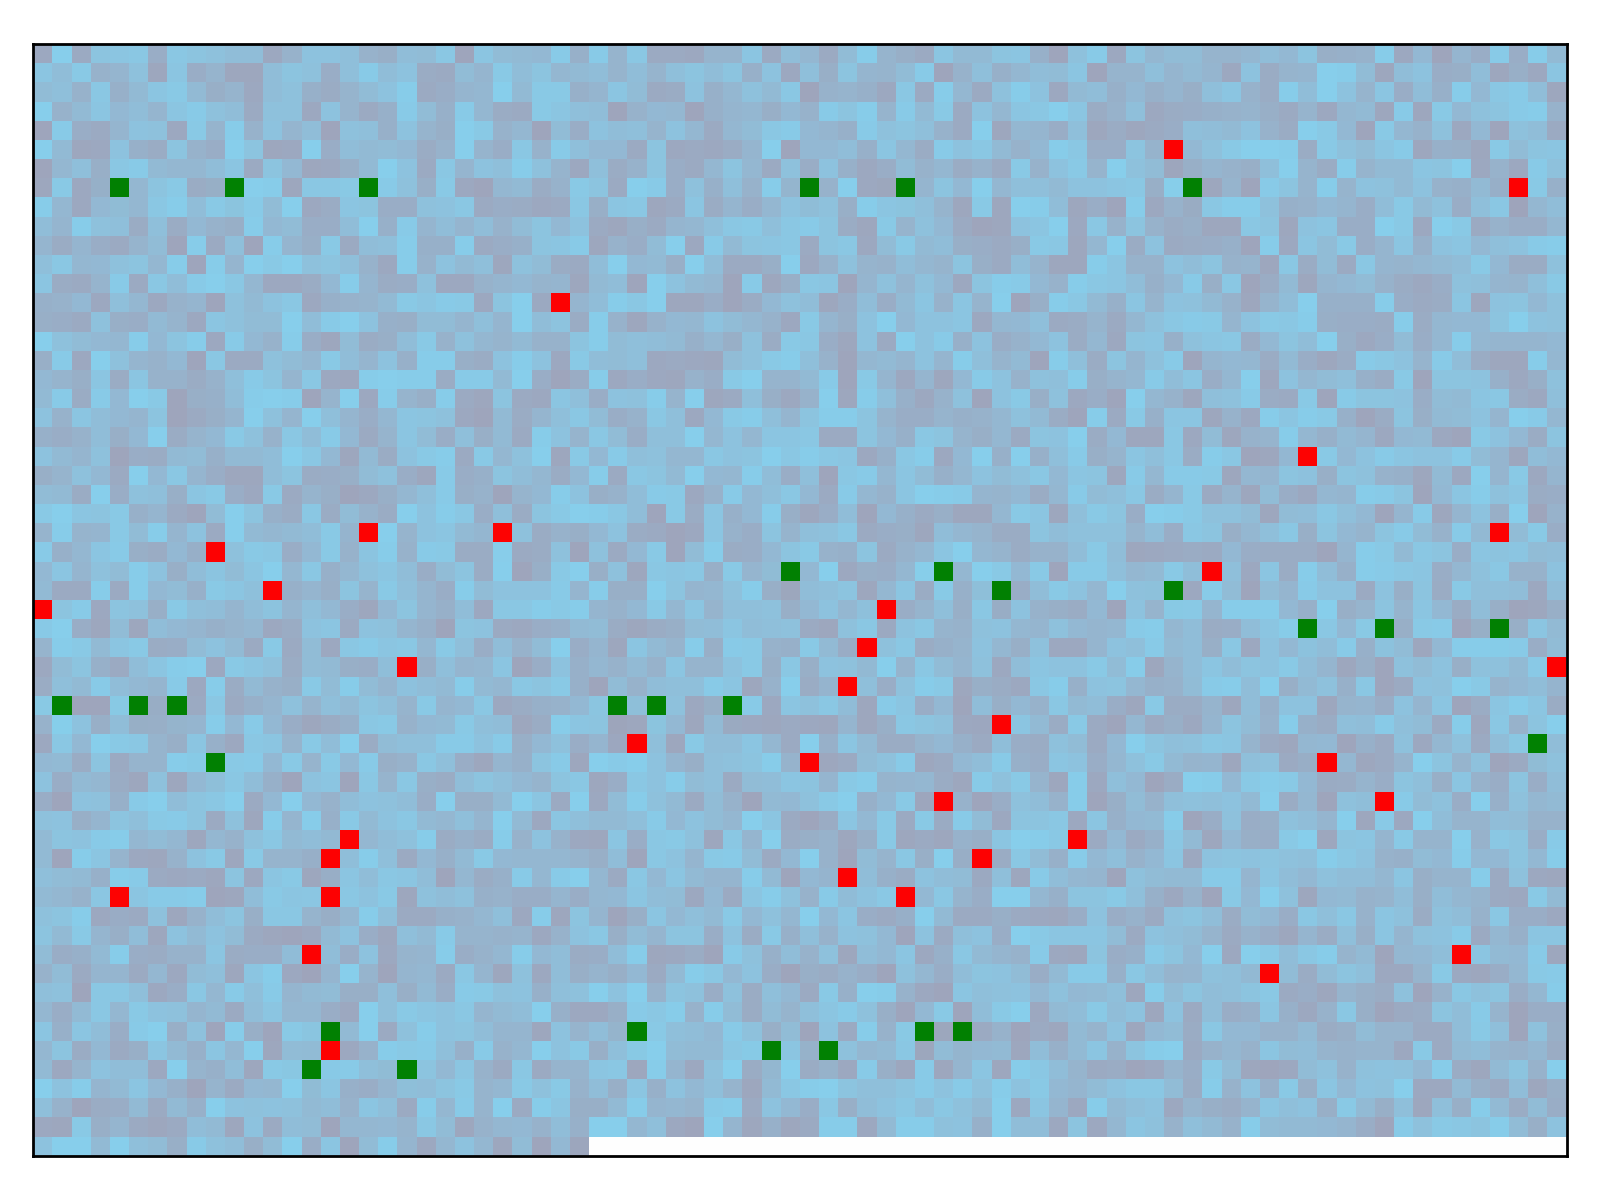
\includegraphics[width=0.75\textwidth]{doc11358_topic0.png} %&
        % 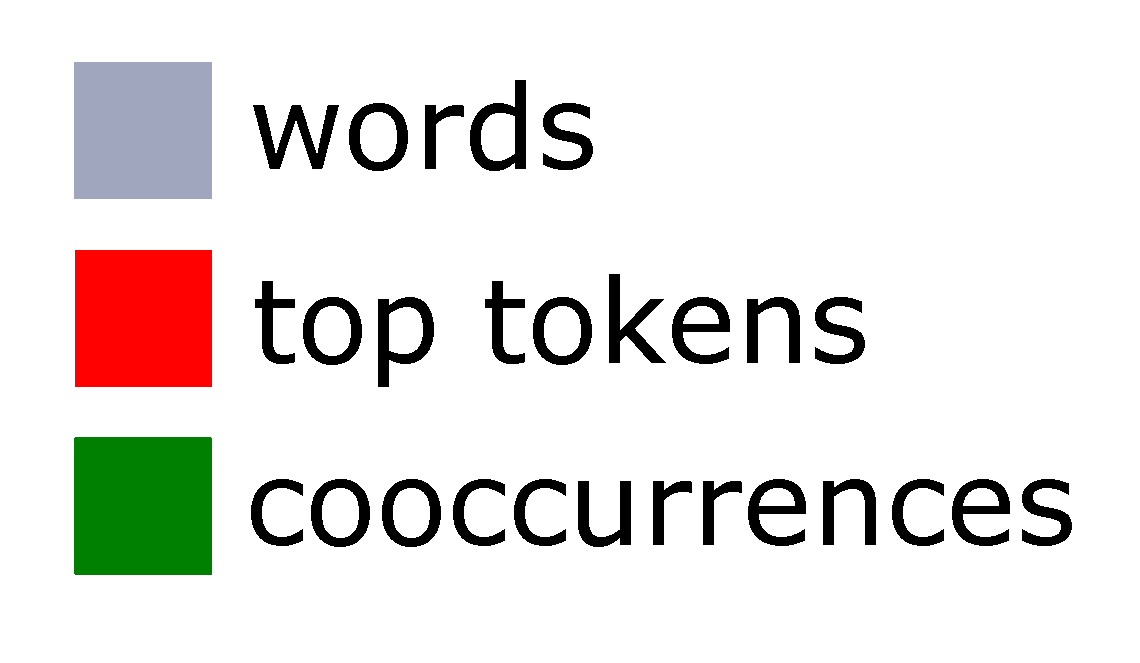
\includegraphics[width=0.25\textwidth]{legend.eps} \\
    %\end{tabular}
\end{figure}
\vspace{-7pt}
Словопозиции обозначены серо-синим цветом, словопозиции верхних слов показаны красным цветом, зелёным цветом показаны словопозиции, имеющие ненулевой вклад в расчёт когерентности (т.е. попадающие в скользящее окно вместе с другим верхним словом).
\end{frame}

\begin{frame}{Доля текста, покрытая верхними словами}

\begin{table}[ht]
\begin{tabular}{|l|l|l|} \hline
         & ПостНаука & Википедия \\ \hline
Минимум  & 0.0159\%  & 0.0065\%  \\ \hline
Медиана  & 0.0483\%  & 0.0293\%  \\ \hline
Среднее  & 0.0619\%  & 0.0356\%  \\ \hline
Максимум & 0.2764\%  & 0.1149\%  \\ \hline
Суммарно & 1.2027\%  & 1.6585\%  \\ \hline
\end{tabular}
\end{table}
      Доля коллекции, имеющая ненулевой вклад в счётчики парных сочетаемостей 10 верхних слов. Статистики посчитаны по каждой теме отдельно; строка <<суммарно>> показывает представительность объединённого множества верхних слов всех тем.
\end{frame}


\begin{frame}{Внутритекстовая когерентность}

\begin{figure}
    \centering
    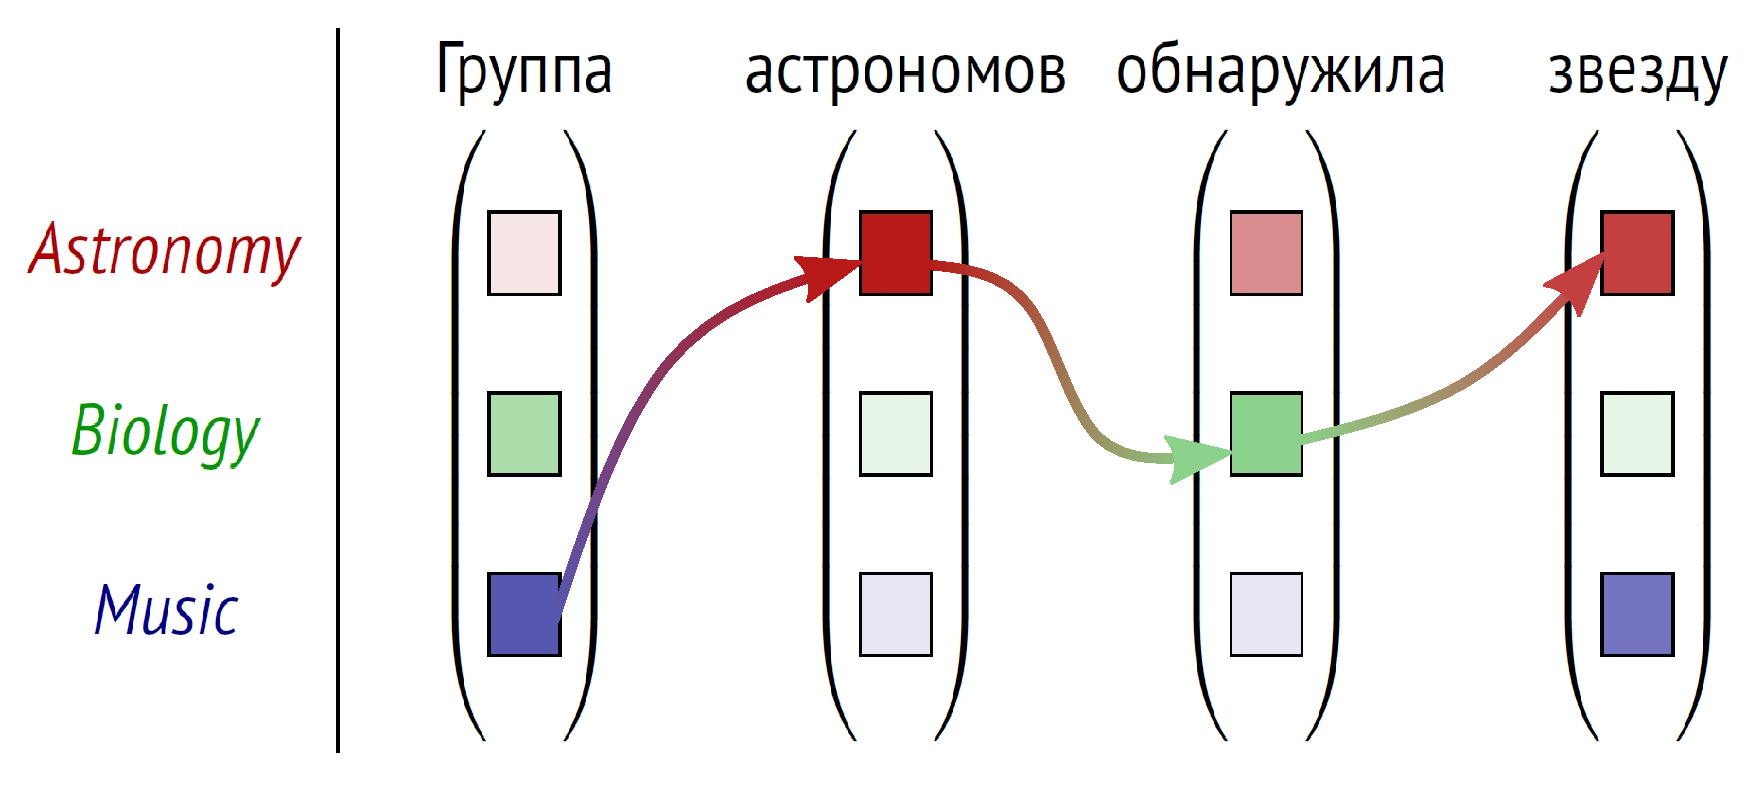
\includegraphics[width=0.8\textwidth, height=0.3\textheight]{astronomers_focon.eps} % .eps image is wrong scaled
\end{figure}

Идея: выделить все соседние слова текста и анализировать их распределение $\phi_{wt}$.
\medskip
(вместо того, чтобы выделять небольшое множество слов при помощи $\phi_{wt}$ и затем анализировать, как эти слова встречаются в тексте)

\end{frame}

\begin{frame}{относительные коэффициенты}
Общие формулы:
\[
\theta_{td} = \norm_{t \in T} \Bigg(
    n_{td} + \sum_{i=1}^k \lambda_i \Big[
        \frac{n}{\sum_{d\in D} r_{id}}
        \Big]
    \theta_{td} \frac{\partial R_i}{\partial \theta_{td}}
\Bigg)
\]



\[
\phi_{wt} = \norm_{w \in W}\Bigg(
    n_{wt} + \sum_{i=1}^k \lambda_i \Big[
        \frac{n}{\sum_{t\in T} r_{it}}
        \Big]
    \phi_{wt} \frac{\partial R_i}{\partial \phi_{wt}}
\Bigg)
\]

\small
\begin{itemize}
    \item { $r_{id} = \sum_{t\in T} \Big | \theta_{td} \frac{\partial R_i}{\partial \theta_{td}} \Big | $ --- воздействие регуляризатора на документ}

    \item{$r_{it} = \sum_{w\in W} \Big| \phi_{wt} \frac{\partial R_i}{\partial \phi_{wt}} \Big| $ --- воздействие регуляризатора на тему}
	\item { $\lambda_i$ - относительный коэффициент регуляризации, показывающий, \emph{во сколько раз} соответствующий регуляризатор влияет на оценку матриц больше, чем коллекция}
\end{itemize}

Случай $\phi_{wt}$ реализован в BigARTM, случай $\theta_{td}$~--- нет (поскольку $r_{id}$ недоступен при параллельной реализации).

\end{frame}

\begin{frame}{Сглаживание и разреживание}
Для регуляризаторов сглаживания/разреживания ($\Phi$ или $\Theta$) формула существенно упрощается!

\begin{table}[]
\begin{tabular}{l|c|c|}
         & \multicolumn{2}{c}{Управляющий параметр}                                                                                                      \\ \hline
         & $\tau$                                          & $\lambda$                                                                                   \\ \hline 
         &    &          \\[-5pt]
$\Phi$   & $\phi_{wt} = \norm_{w \in W}\Bigg(n_{wt} + \tau\Bigg)$    & $\phi_{wt} = \norm_{w \in W}\Bigg(n_{wt} + \lambda {\color{red}\frac{n}{|W||T|}}\Bigg)$    \\[15pt] \hline
         &    &          \\[-5pt]
$\Theta$ & $\theta_{td} = \norm_{t \in T} \Bigg(n_{td} + \tau\Bigg)$ & $\theta_{td} = \norm_{t \in T} \Bigg(n_{td} + \lambda {\color{red}\frac{n}{|D| |T|}}\Bigg)$ \\[15pt]  \hline
\end{tabular}
\end{table}
Вывод: сглаживание/разреживание с абсолютным коэффициентом и относительным эквивалентно 

\small
(в частности, можно вычислить абсолютный коэффициент сглаживания $\Theta$, эквивалентный заданному относительному ).

\end{frame}

\begin{frame}{репараметризация сглаживания/разреживания}
	
\begin{equation}
\tau = \frac{n}{|D| \cdot |T|} \frac{\lambda}{(1-\lambda)}
\end{equation}

\begin{equation}
\tau = \frac{n}{|T|\cdot|W|} \frac{\lambda}{(1-\lambda)}  
\end{equation}

Интерпретация: берём $\lambda$ частей априорного распределения
\[
\frac{1}{|T|}\text{ или }\frac{1}{|W|}
\]
и $(1-\lambda)$ частей от оценки максимума правдоподобия 
\[
\frac{n_{td}}{n_d}\text{ или }\frac{n_{wt}}{n_t}
\]


\end{frame}

\begin{frame}{относительные веса модальностей}
Формула общего правдоподобия для мультимодального случая:

\[
L(\Phi^m, \Theta) = \sum_m \tau_m \sum_{d\in D} \sum_{w \in W^m} n_{dw} \ln p(w \cond d) \rightarrow \max, 
\]

где коэффициенты $\tau_m$ показывают \textit{вес} модальности $m$. Проинтерпретируем это выражение как введение $M-1$ дополнительного регуляризатора $\Theta$ с коэффициентами $\tau_m$. Тогда $\frac{n}{\sum_{d\in D} r_{id}}$ тоже выражается через константы, известные ещё на этапе построения коллекции:

\[
\tau_m = \lambda_m \frac{n}{\sum_d \check{n}_d^{(m)}} \iff
\lambda_m = \tau_m \frac{\sum_d \check{n}_d^{(m)}}{n}
\]

\end{frame}


\begin{frame}{Второстепенность матрицы Тета}

Матрица $\Theta$ является менее важной, чем $\Phi$ и на практике хочется её не хранить, а восстанавливать <<на лету>>.

\begin{itemize}
\item В процессе оценки интерпретируемости обычно используется только матрица $\Phi$.

\item Динамическое расширение коллекции документов: сильно увеличивается $|D|$, $|W|$ растёт медленнее.

\item Пакетный EM-алгоритм: разные документы обрабатываются разными потоками. Используется $\theta_d$, а не матрица $\Theta$ целиком.
\end{itemize}

\bigskip
По этим соображениям явно введём зависимость $\Theta = f(\Phi)$. Таким образом, мы предлагаем заменить исходную оптимизационную задачу на следующую:

\begin{equation} \label{eq:tEM}
L(\Phi, f(\Phi) ) + R(\Phi, f(\Phi) ) \to \max_{\Phi},
\end{equation}
\end{frame}

\begin{frame}[t]{$\Theta$ может скомпенсировать <<плохую>> $\Phi$}

Коллекция из 3 документов: 
\begin{figure}[t]
\begin{minipage}[t]{0.4\textwidth}
	\medskip
\begin{itemize}
    \item \texttt{herbs and spices}
    \item \texttt{spices and medicine}
    \item \texttt{herbs and medicine}
\end{itemize}
	\end{minipage}
	% $\qquad\quad$
	\begin{minipage}[t]{0.4\textwidth}
\begin{center}
\begin{tabular}{l|llll}
$n_{dw}$   & and & herbs & spices & medicine \\ \hline
doc1       & 1   & 1     & 1      & 0        \\
doc2       & 1   & 0     & 1      & 1        \\
doc3       & 1   & 1     & 0      & 1      
\end{tabular}
\end{center}

\end{minipage}
\end{figure}

Есть много локальных оптимумов с зашумлённой $\Phi$, недостатки которой  <<спрятаны>>  при помощи нулей в матрице $\Theta$:
\small
\begin{minipage}[t]{0.4\textwidth}
\[
\Phi =
\begin{pmatrix}
    0.044 & 0.956 & 0 & 0 \\
    0.488 & 0 &  0 & 0.512 \\
    0.488 & 0 & 0.512 & 0   \\
    0.281 & 0 & 0.279 & 0.44 \\
\end{pmatrix},
\]
	\end{minipage}
	$\qquad\quad$
	\begin{minipage}[t]{0.4\textwidth}
\[
\Theta =
\begin{pmatrix}
    0.349 & 0 & 0.651 & 0 \\
    0 & 0.008 & 0.244 & 0.748 \\
    0.348 & 0.652 & 0 & 0 \\
\end{pmatrix}.
\]
\end{minipage}
\bigskip
\[
\Phi \cdot \Theta \approx \frac{1}{3} n_{dw}
\]
\normalsize
\end{frame}

\begin{frame}{EM-алгоритм при $\Theta=f(\Phi)$ [Ирхин, 2020]}
\small
\begin{Theorem}
    Пусть функция $R(\Phi,\Theta)$ непрерывно дифференцируема, а $\Theta$ находится в функциональной зависимости от $\Phi$ согласно формуле    $\theta_{td}(\Phi)
    = \norm_{t\in T} \biggl( \sum_{w\in W} n_{dw} p_{tdw} \biggr)$.
    Тогда точка $\Phi$ локального максимума 
    удовлетворяет системе уравнений со вспомогательными переменными $h_w,\ \theta_{td},\ p_{tdw},\ c_{td},\ \gamma_{dw}$:
\begin{align*}
    \phi_{wt} = \norm_{w\in W}
        \Biggl(\,&
        \sum_{d\in D} n_{dw} p_{tdw} \\
        + &\underbrace{\sum_{d\in D} n_{dw} n_d^{-1} \phi_{wt}h_w (c_{td}-h_w\gamma_{dw})}_{
            \let\scriptstyle\textstyle
            \substack{\textup{очень похоже на регуляризатор}}
        } \\ 
        + &\underbrace{
            \phi_{wt} \frac{\partial{R}}{\partial{\phi_{wt}}}
          }_{
          \let\scriptstyle\textstyle
            \substack{\textup{регуляризатор}}
        }
        \Biggr)
\end{align*}
\end{Theorem}

\normalsize
\end{frame}

\begin{frame}{Влияние на тематическую модель}

\begin{figure}
\setlength\tabcolsep{0pt} % default value: 6pt
\begin{tabular}{cc}
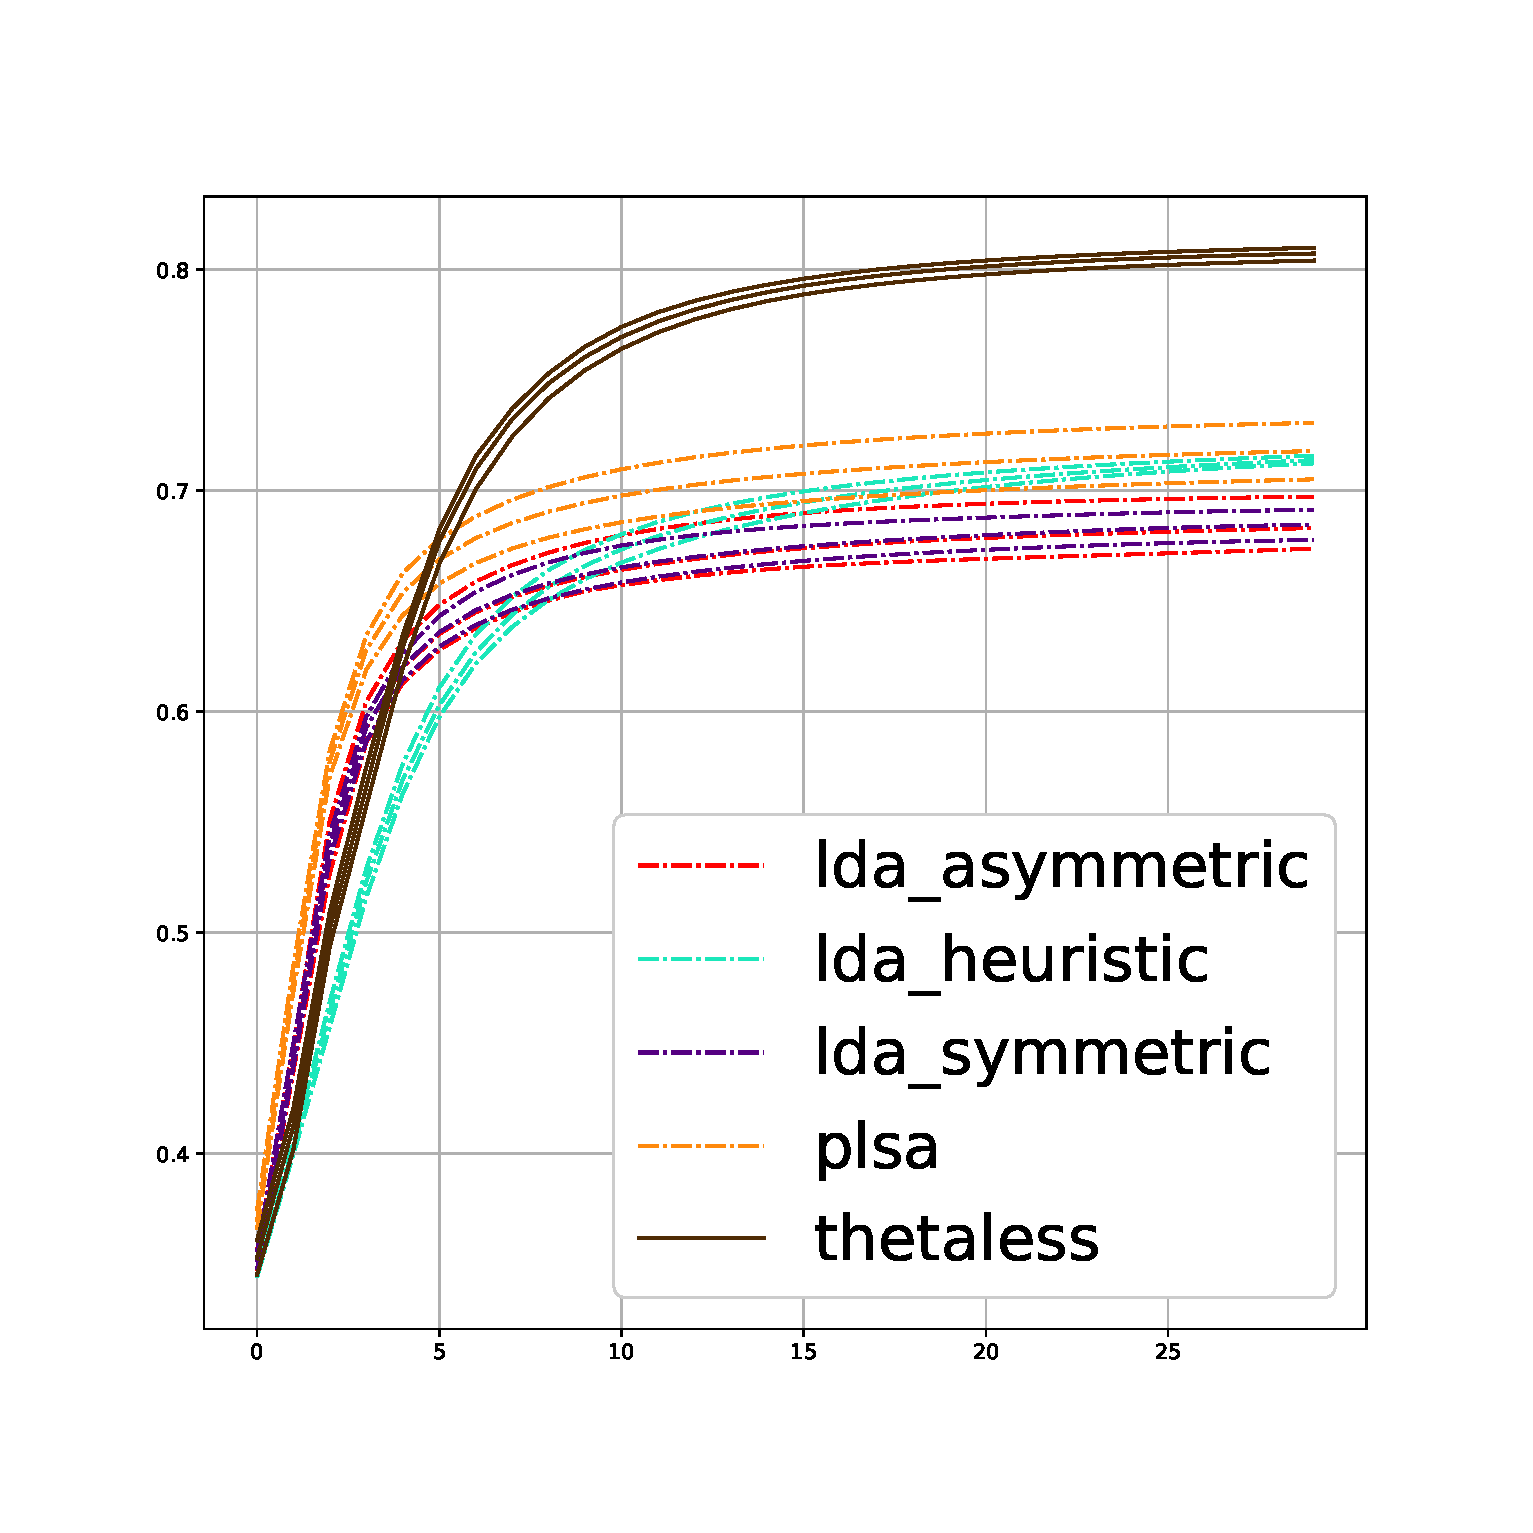
\includegraphics[width=54mm]{images/CH4_baselines_diversity_jensenshannon_False.eps}
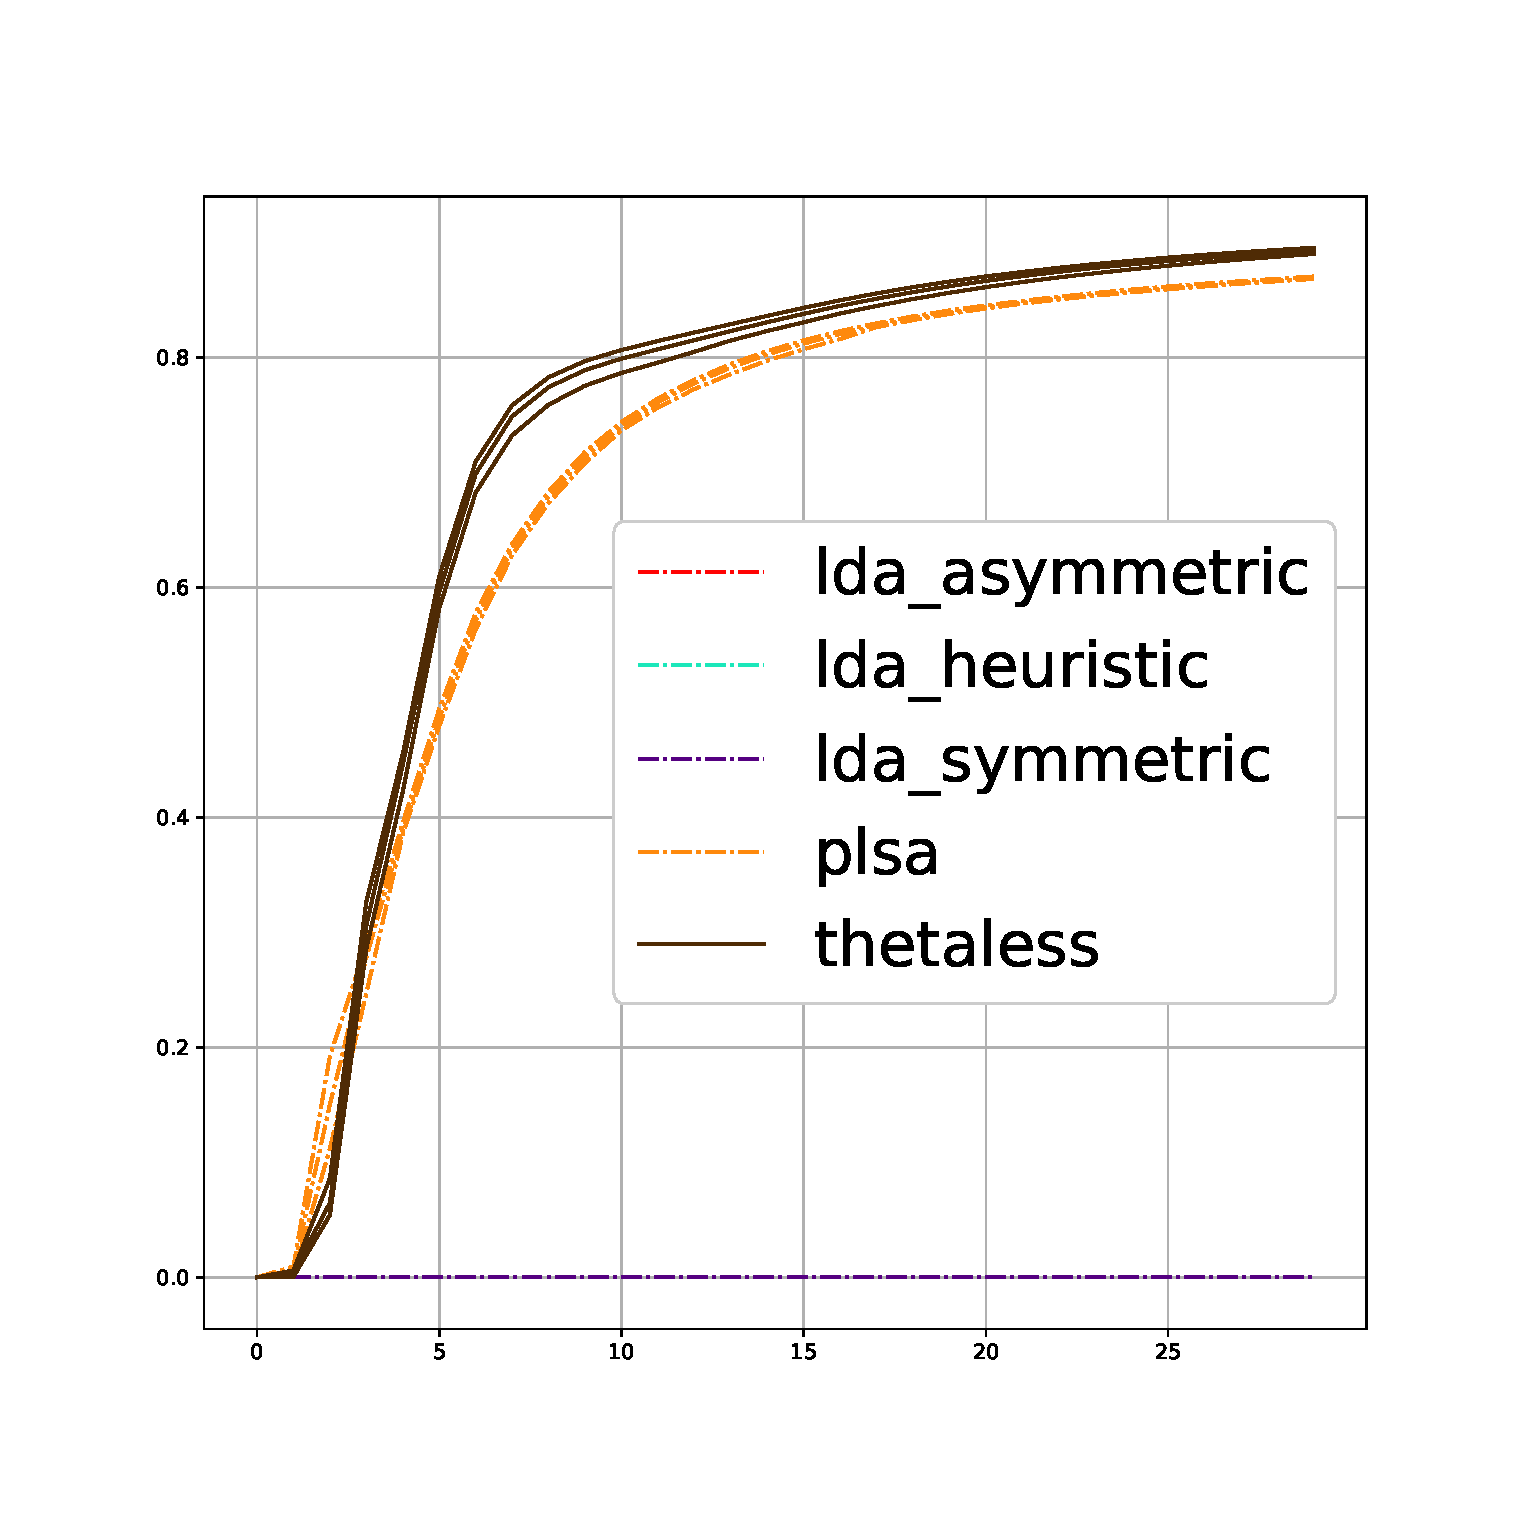
\includegraphics[width=54mm]{images/CH4_baselines_SparsityPhiScore.eps}& \end{tabular}
\end{figure}
Сравнение с базовыми моделями (PLSA и LDA с 3 видами приоров). Каждой модели соответствуют три линии: среднее значение, минимум и максимум (по пяти случайным перезапускам)
\end{frame}

\begin{frame}{Влияние на тематическую модель}

\begin{figure}
\setlength\tabcolsep{0pt} % default value: 6pt
\begin{tabular}{cc}
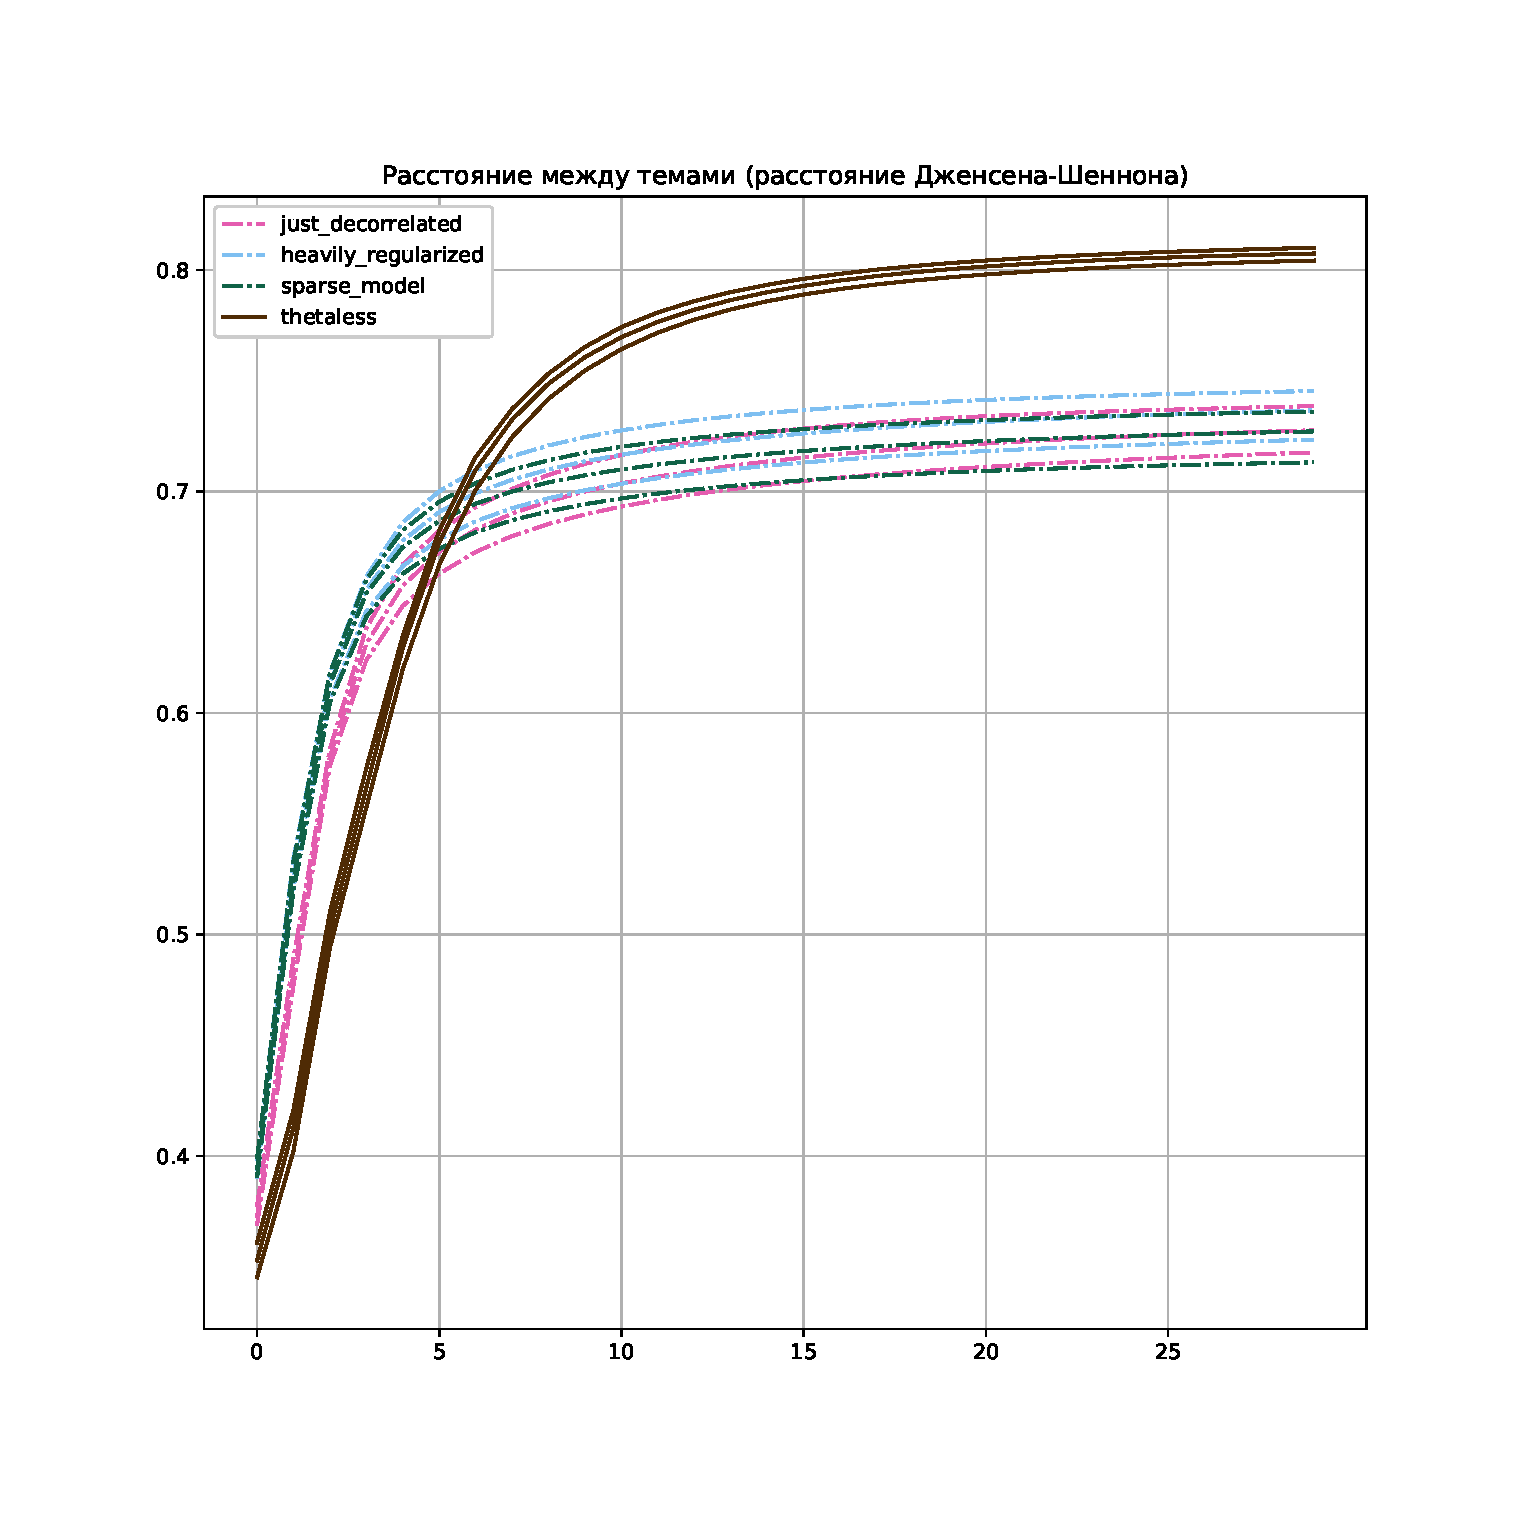
\includegraphics[width=54mm]{images/CH4_vs_regularized_diversity_jensenshannon_False.eps}
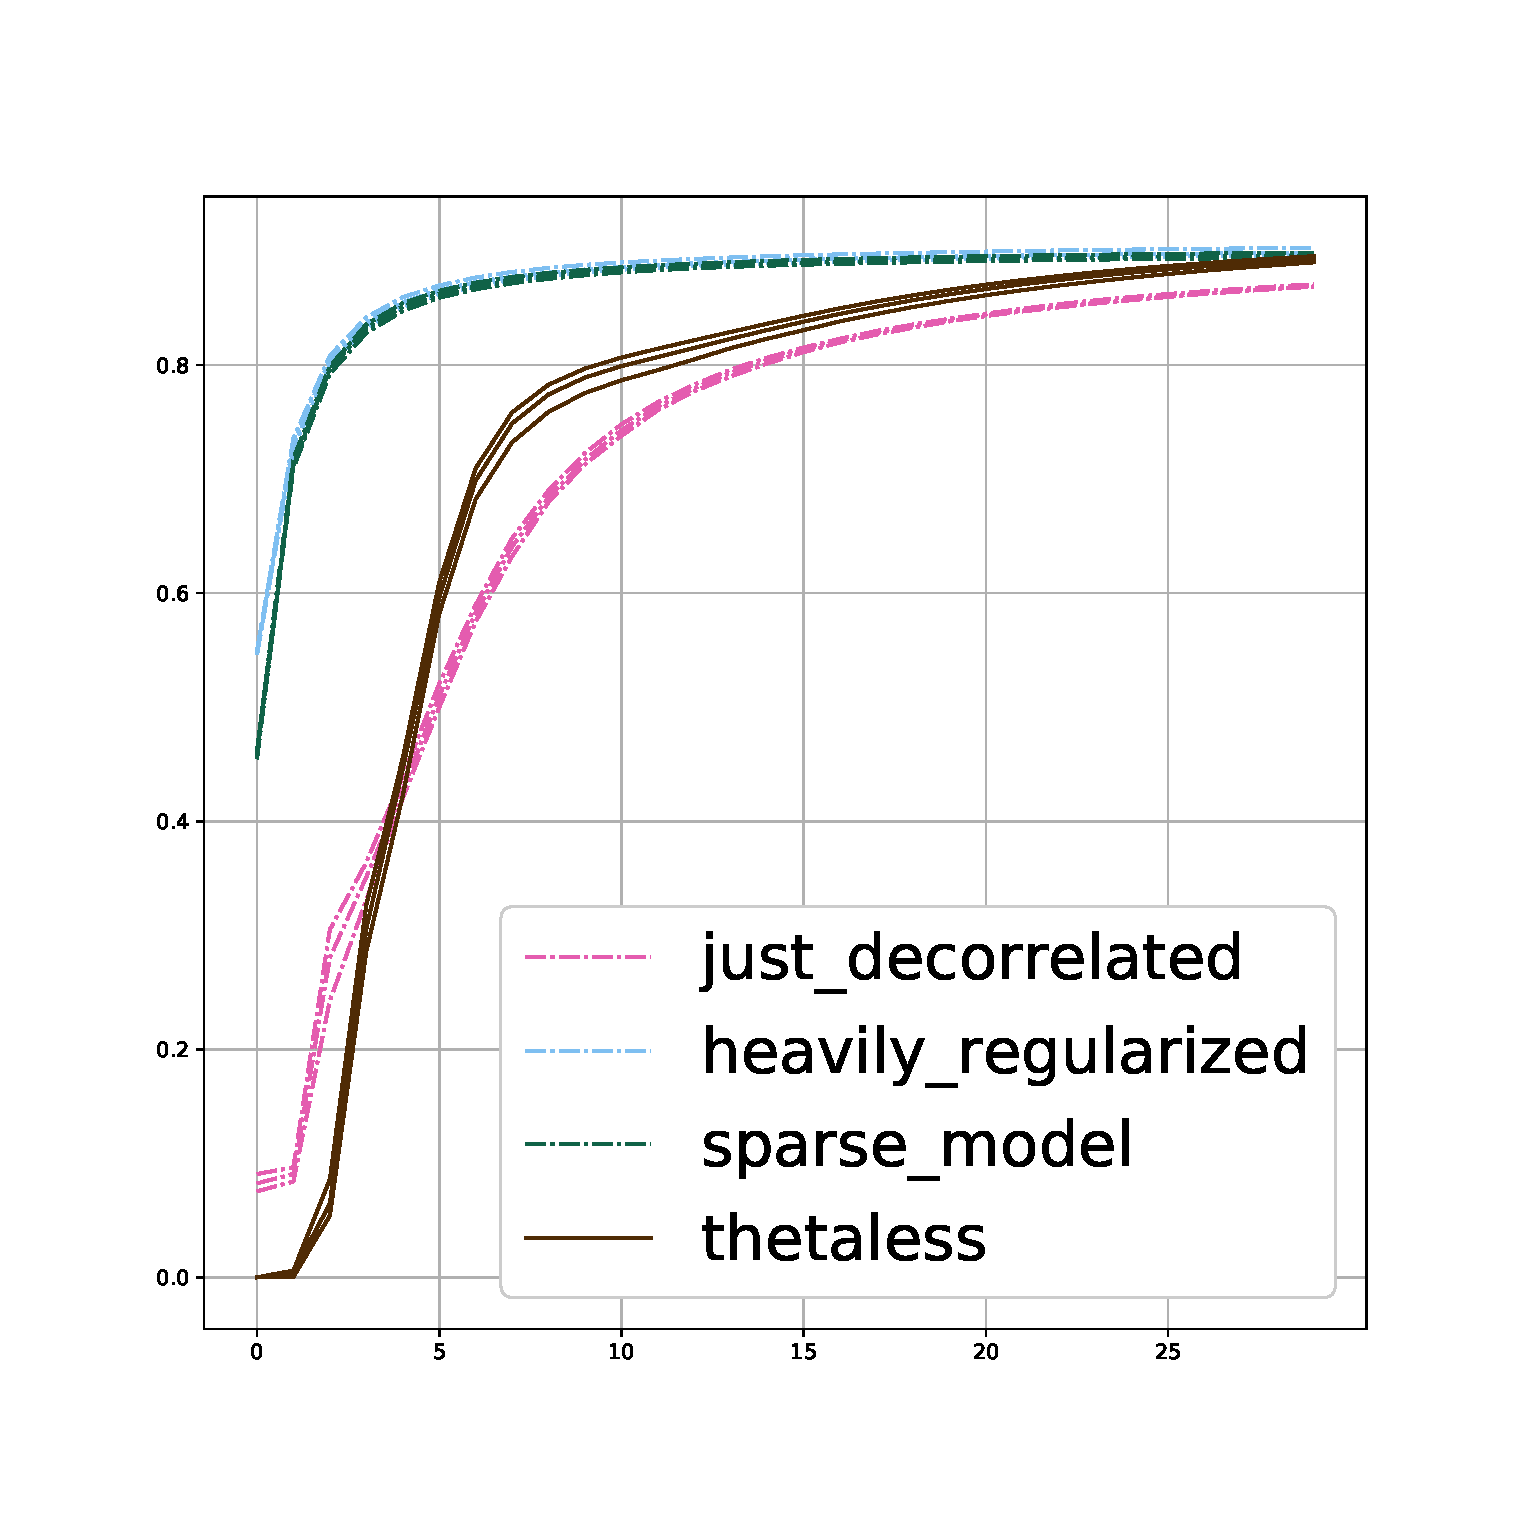
\includegraphics[width=54mm]{images/CH4_vs_regularized_SparsityPhiScore.eps}& \end{tabular}
\end{figure}
Сравнение с тремя аддитивно регуляризованными моделями
\end{frame}

\begin{frame}{Комбинирование с другими регуляризаторами}

\begin{figure}
\setlength\tabcolsep{0pt} % default value: 6pt
\begin{tabular}{cc}
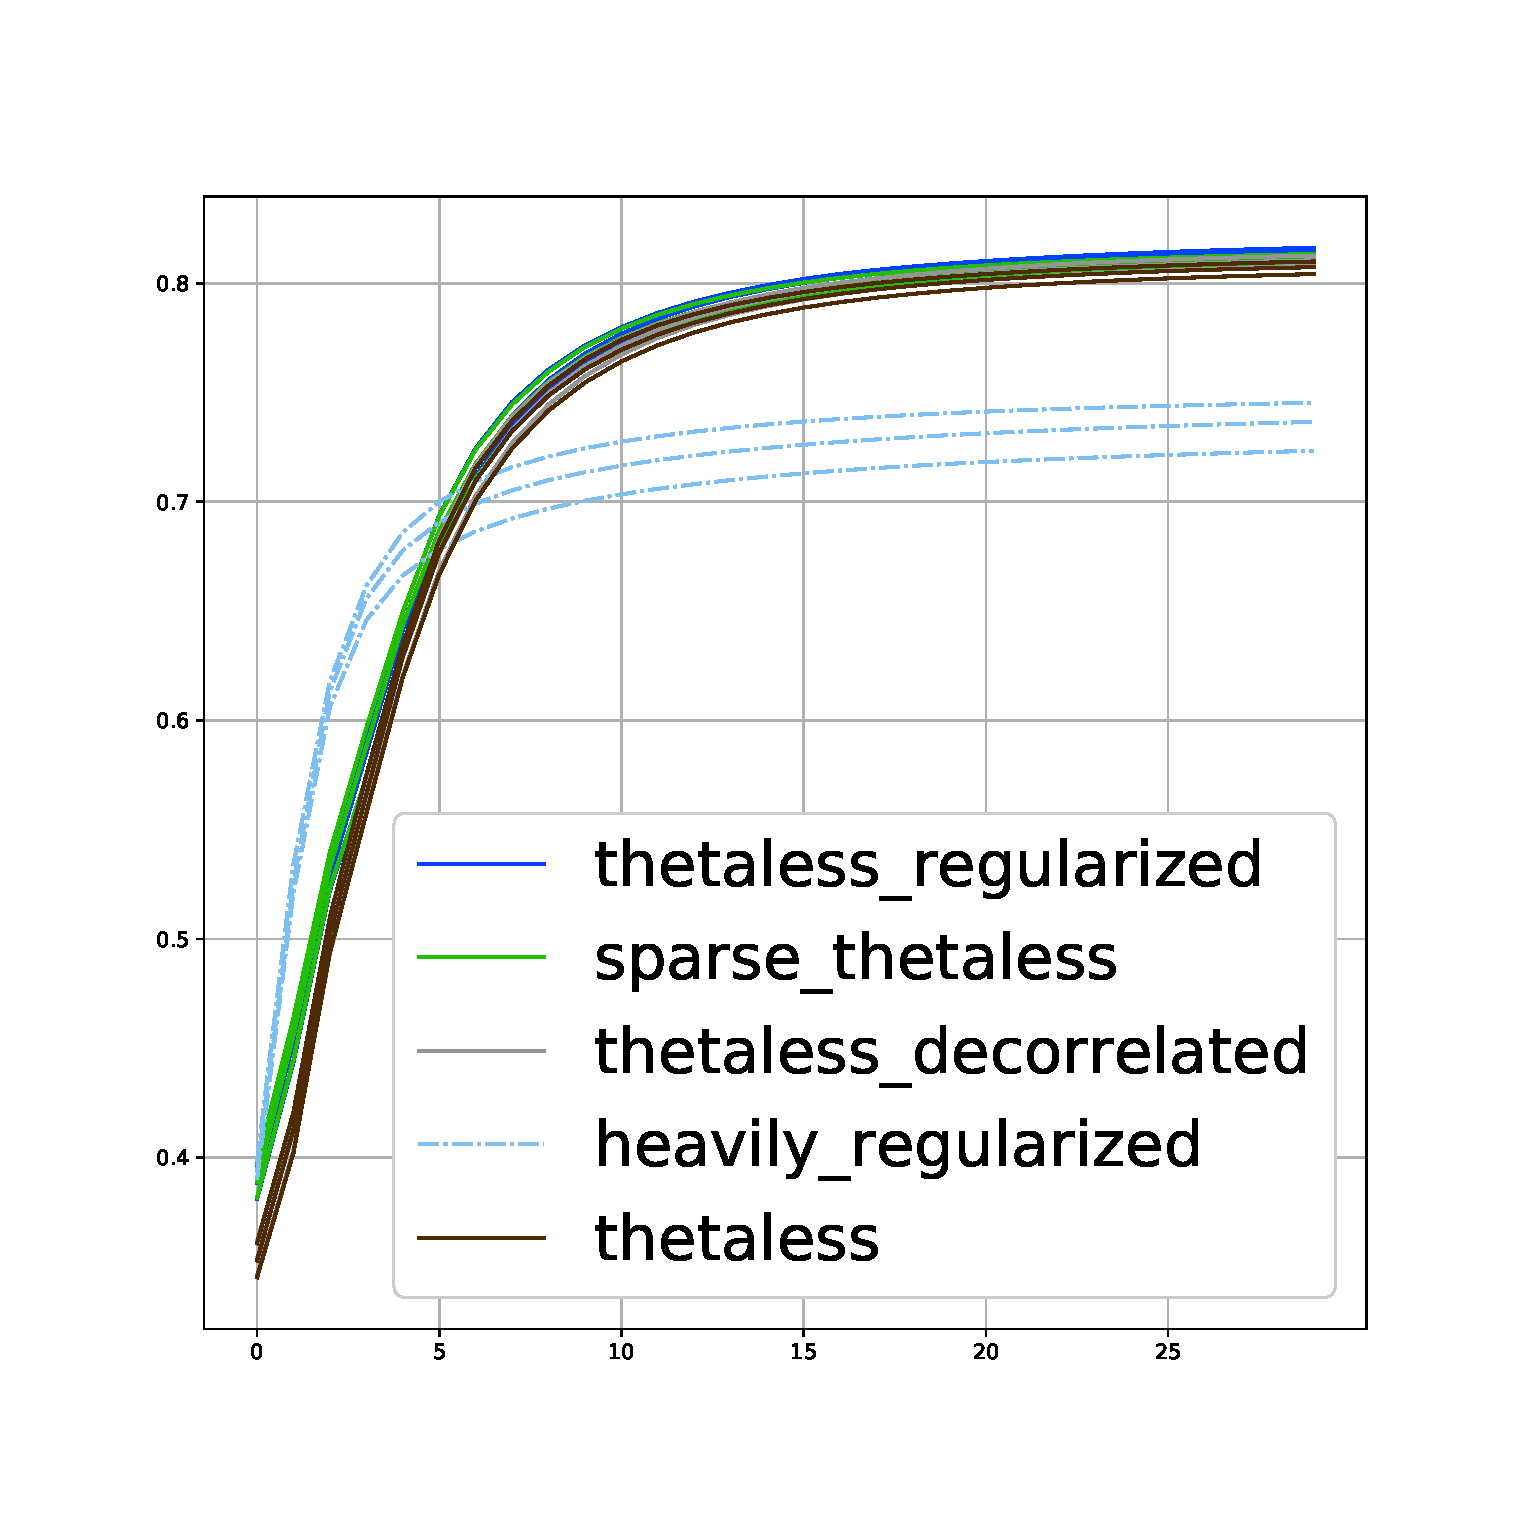
\includegraphics[width=54mm]{images/CH4_improved_diversity_jensenshannon_False.eps}
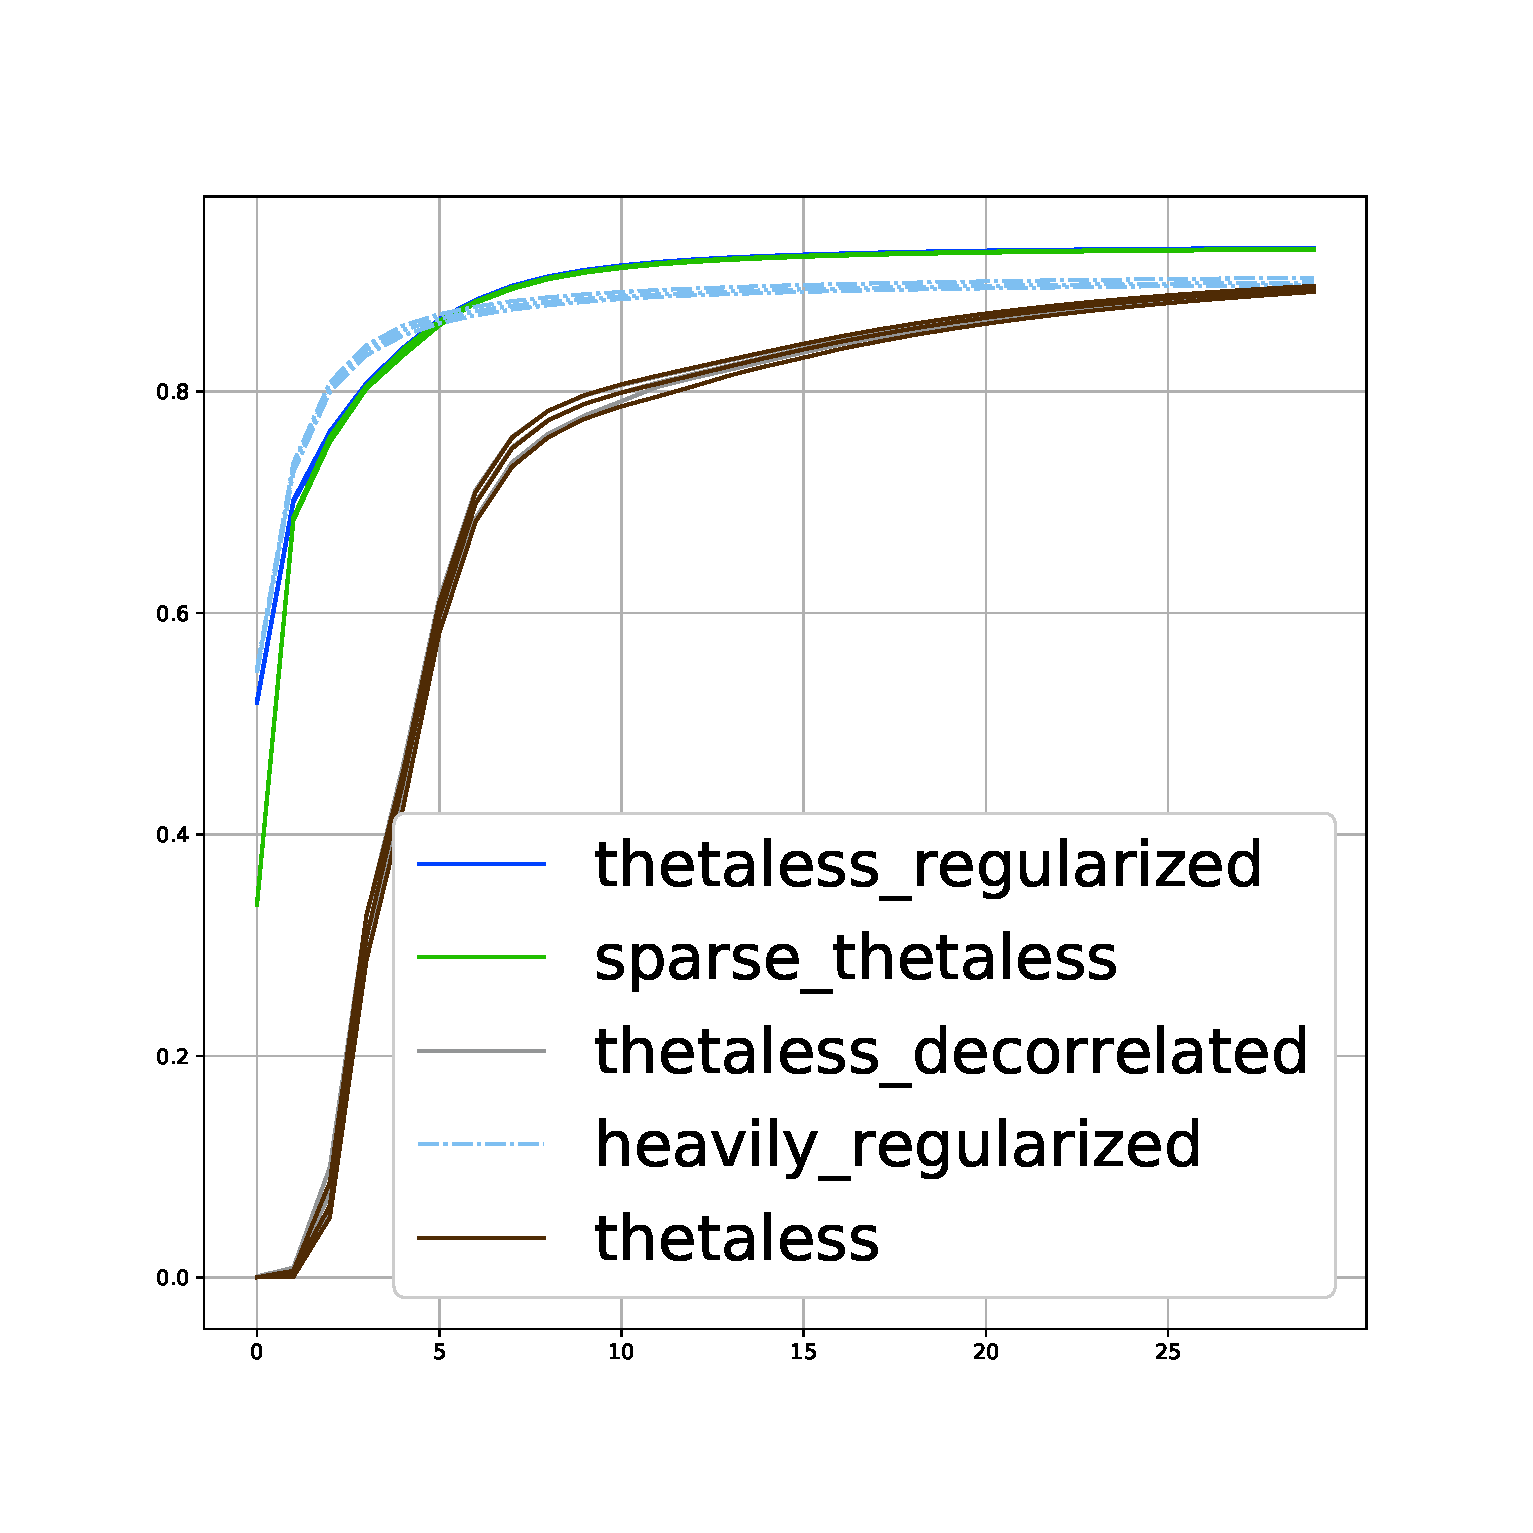
\includegraphics[width=54mm]{images/CH4_improved_SparsityPhiScore.eps}& \end{tabular}
\end{figure}
\end{frame}


\begin{frame}{Библиотека TopicNet}

\begin{figure}[ht]
    \centering
    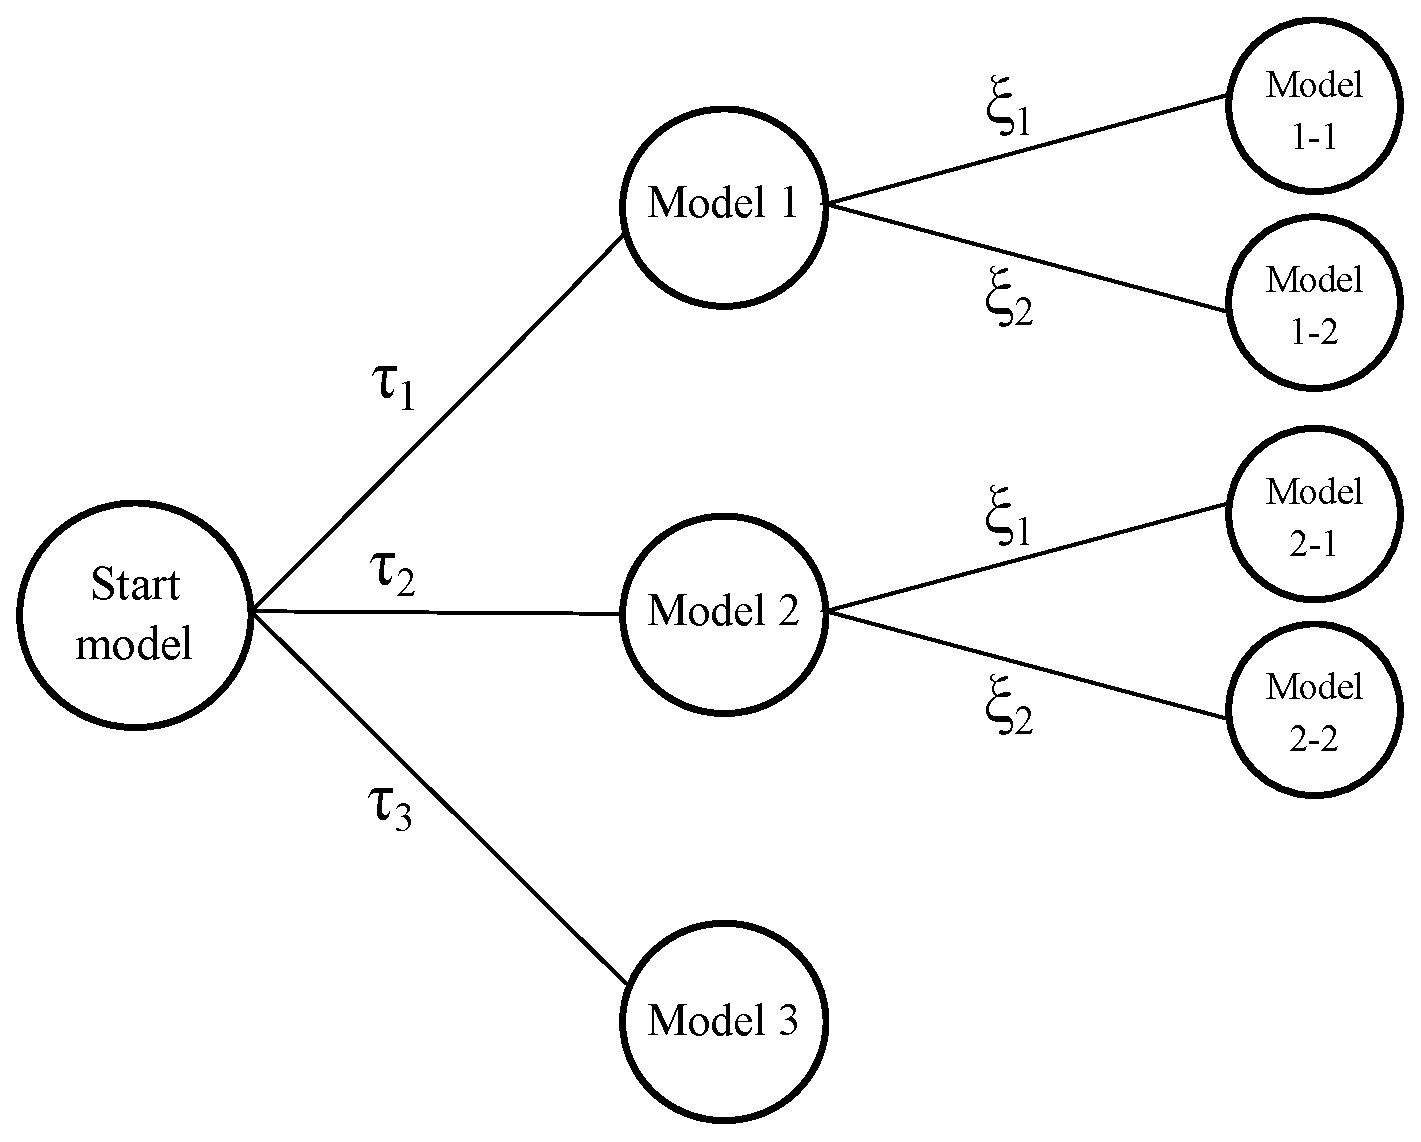
\includegraphics[width=0.7\textwidth]{training_scheme_example.eps}
\end{figure} 
	Тут будет про дерево эксперимента и кубы
\end{frame}



\begin{frame}{Библиотека TopicNet}

\begin{figure}[ht]
% \footnotesize
\raggedright
\texttt{TopicKernel@word.average\_contrast > 0.95 * MAXIMUM( \\
\hphantom{\ \ \ \ \ \ \ \ }TopicKernel@word.average\_contrast) \\
\hphantom{\ \ } and PerplexityScore@all < 1.1 * MINIMUM( \\
\hphantom{\ \ \ \ \ \ \ \ }PerplexityScore@all) \\
\hphantom{\ \ } and SparsityPhiScore@word -> max\\
\hphantom{\ \ } COLLECT 3} \\
\label{DSL-example}
\end{figure} 
	Язык отбора моделей:
	
%\begin{lstlisting}
%S -> <Expr> | <Expr> <Clct>
%<Clct> -> COLLECT <Int>
%<Expr> -> <Expr> AND <Expr>
%<Optr> -> less | eq | great
%<Expr> -> <Literal> <Optr> <Number>
%<Expr> -> <Literal> to MIN | <Literal> to MAX
%<Literal> -> <ScoreName> | model<ParameterName>
%\end{lstlisting} 

\texttt{model.num\_topics == 10 AND SparsityPhiScore\@word > MEDIAN(SparsityPhiScore\@word) AND MyCustomScore -> MAX}

\end{frame}

\begin{frame}{Библиотека TopicNet}
	Тут будет про рецепты и конфиги в YAML-формате
\end{frame}

\begin{frame}{TopicNet vs GenSim}
	круто по LogLift и различности, но не дожали по когерентности
\end{frame}

\begin{frame}{TopicNet Thetaless vs GenSim}
Вспоминаем, что Thetaless повышает когерентность. Добавляем. Победили по всему.
\end{frame}


\begin{frame}{Таксономия обращений}
	Постановка задачи
\end{frame}

\begin{frame}{Таксономия обращений}
	Две разных коллекции. Примеры документов/тем из первой и из второй.
\end{frame}

\begin{frame}{Таксономия обращений}
    мы использовали пять модальностей
    среди них нграмы
	веса модальностей относительные: чиселки.
\end{frame}

\begin{frame}{Таксономия обращений}
	примеры тем модели

	можно гифку с иерархией тем?
\end{frame}

\begin{frame}[t]{Публикации и РИДы}
\footnotesize

Публикации в изданиях, индексируемых Scopus:
\begin{itemize}
    \smallskip\item  V. Alekseev, V. Bulatov, K. Vorontsov. Intra-text coherence as a measure of topic models’ interpretability  // Dialogue 2018

    \smallskip\item A. Popov, V. Bulatov, D. Polyudova, E. Veselova. Unsupervised dialogue intent detection via hierarchical topic model // RANLP 2019

    \smallskip\item V. Bulatov, V. Alekseev, K. Vorontsov, D. Polyudova, E. Veselova, A. Goncharov, E. Egorov. TopicNet: Making Additive Regularisation for Topic Modelling Accessible // LREC 2020

    \smallskip\item\color{red} И. А. Ирхин, В. Г. Булатов, К. В. Воронцов. Аддитивная регуляризация тематических моделей с быстрой векторизацией текста // Компьютерные исследования и моделирование, 2020
\end{itemize}

Зарегистрированные программы для ЭВМ в РФ:
\begin{itemize}
    \smallskip\item  Topic Net Cooking Machine  / Гончаров А. В., Булатов В. Г., Воронцов. К. В.; МФТИ. --- опубл. 17.09.2019, 2019662102

    \smallskip\item Система создания таксономии текстовой коллекции диалогового контактного центра / Гончаров А. В., Егоров. Е. О., Веселова. Е. Р., Булатов. В. Г.; МФТИ. --- опубл. 17.03.2020, 2020613851

    \smallskip\item Topic Net Viewers  / Гончаров А. В., Булатов В. Г., Воронцов. К. В.; МФТИ. --- опубл. 10.09.2019, 2019661840

\end{itemize}

\normalsize
\end{frame}


       % Настройки заглавной странице
% \begin{frame}
    \frametitle{Научная новизна}
    \begin{itemize}
        \item Впервые реализован \dots
        \item Разработана программа \dots
        \item Впервые проведён анализ \dots
        \item Предложена схема \dots
    \end{itemize}
\end{frame}
\note{
    Проговаривается вслух научная новизна
}

\begin{frame}
    \frametitle{Научная и практическая значимость}
    \begin{itemize}
        \item Получены выражения для \dots.
        \item Определены условия \dots.
        \item Разработаны устройства \dots.
    \end{itemize}
\end{frame}
\note{
    Проговариваются вслух научная и практическая значимость
}

\begin{frame}[plain, noframenumbering] % последний слайд без оформления
    \begin{center}
        \Huge
        Спасибо за внимание!
    \end{center}
\end{frame}
    % Последние слайды презентации
% \appendix
% 

\includepdf[pages=-,scale=.8,offset=0 -25,pagecommand={
    \chapter{Свидетельства о государственной регистрации программ}\label{app:A}
}]{Documents/Taxonomy_2020613851.pdf}

\includepdf[pages=-,scale=.8,offset=0 -25]{Documents/Topic Net Cooking Machine 2019662102.pdf}

\includepdf[pages=-,scale=.8,offset=0 -25]{Documents/Topic Net Viewers 2019661840.pdf}
      % Запасные слайды презентации
\end{document}
